% REPORT.TEX - University of Warwick Reports / Dissertations / Projects
% 
% Author - Chris Quinn 28/06/2020
% 
%
% A template for students and masters dissertations, flexible for your
% needs.
%
% This is the main .tex which will tell the compiler to include everything, 
% each chapter/section is then in folders for convenience, as you include more awid
% images it can get harder and harder to manage.
%
% First things first, declaration of the document class along with the packages % we need.


\documentclass[pdftex,11pt,a4paper,oneside]{article}
%Can change the pt, papersize etc.

\usepackage{amsmath} %For both in-line and equation mode
\numberwithin{equation}{section} %Numbering of our equations per section
\usepackage{algorithm}
\usepackage{algorithmic} %Algorithm styles, need to be nested for the example shown
\usepackage{fancyhdr} %For our headers
\usepackage{graphicx} %Inserting images
\usepackage{setspace} %Spacing on the front page for crest and titles
\usepackage[]{fncychap} % Styles can be Sonny, Lenny, Glenn, Conny, Rejne, Bjarne and Bjornstrup
\usepackage[hyphens]{url} %Deals with hyphens in urls to make them clickable
\usepackage{xcolor} %Great if you want coloured text
\usepackage{tabularx}
\usepackage{appendix} %Take a wild guess slick
\usepackage{caption}
\usepackage{booktabs} % Used for the classification report table
\usepackage{listings}
\usepackage{color}

% Bibliography
\usepackage[backend=biber,style=authoryear-ibid]{biblatex}
\setlength\bibitemsep{\baselineskip}

\definecolor{mygreen}{rgb}{0,0.6,0}
\definecolor{mygray}{rgb}{0.5,0.5,0.5}
\definecolor{mymauve}{rgb}{0.58,0,0.82}

%\lstset{ 
%  backgroundcolor=\color{white},   % choose the background color; you must add \usepackage{color} or \usepackage{xcolor}; should come as last argument
%  basicstyle=\footnotesize,        % the size of the fonts that are used for the code
%  breakatwhitespace=false,         % sets if automatic breaks should only happen at whitespace
%  breaklines=true,                 % sets automatic line breaking
%  captionpos=b,                    % sets the caption-position to bottom
%  commentstyle=\color{mygreen},    % comment style
%  deletekeywords={...},            % if you want to delete keywords from the given language
%  escapeinside={\%*}{*)},          % if you want to add LaTeX within your code
%  extendedchars=true,              % lets you use non-ASCII characters; for 8-bits encodings only, does not work with UTF-8
%  firstnumber=1,                % start line enumeration with line 1000
%  frame=single,	                   % adds a frame around the code
%  keepspaces=true,                 % keeps spaces in text, useful for keeping indentation of code (possibly needs columns=flexible)
%  keywordstyle=\color{blue},       % keyword style
%  language=Octave                 % the language of the code
%  morekeywords={*,...},            % if you want to add more keywords to the set
%  numbers=left,                    % where to put the line-numbers; possible values are (none, left, right)
%  numbersep=5pt,                   % how far the line-numbers are from the code
%  numberstyle=\tiny\color{mygray}, % the style that is used for the line-numbers
%  rulecolor=\color{black},         % if not set, the frame-color may be changed on line-breaks within not-black text (e.g. comments (green here))
%  showspaces=false,                % show spaces everywhere adding particular underscores; it overrides 'showstringspaces'
%  showstringspaces=true,          % underline spaces within strings only
%  showtabs=false,                  % show tabs within strings adding particular underscores
%  stepnumber=1,                    % the step between two line-numbers. If it's 1, each line will be numbered
%  stringstyle=\color{mymauve},     % string literal style
%  tabsize=2,	                   % sets default tabsize to 2 spaces
%  title=\lstname                   % show the filename of files included with \lstinputlisting; also try caption instead of title
%}

\lstset{ 
  backgroundcolor=\color{white},   % choose the background color; you must add \usepackage{color} or \usepackage{xcolor}; should come as last argument
  basicstyle=\footnotesize, % the size of the fonts that are used for the code and the font family
  breakatwhitespace=false,         % sets if automatic breaks should only happen at whitespace
  breaklines=true,                 % sets automatic line breaking
  captionpos=b,                    % sets the caption-position to bottom
  commentstyle=\color{mygreen},    % comment style
  deletekeywords={...},            % if you want to delete keywords from the given language
  escapeinside={\%*}{*)},          % if you want to add LaTeX within your code
  extendedchars=true,              % lets you use non-ASCII characters; for 8-bits encodings only, does not work with UTF-8
  frame=single,                        % adds a frame around the code on top and bottom
  framexleftmargin=10pt,           % adjust the left margin of the frame
  framexrightmargin=10pt,          % adjust the right margin of the frame
  framextopmargin=5pt,             % adjust the top margin of the frame
  keepspaces=true,                 % keeps spaces in text, useful for keeping indentation of code (possibly needs columns=flexible)
  keywordstyle=\color{blue},       % keyword style
  language=Octave,                 % the language of the code
  morekeywords={*,...},            % if you want to add more keywords to the set
  numbers=left,                    % where to put the line-numbers; possible values are (none, left, right)
  numbersep=5pt,                   % how far the line-numbers are from the code
  numberstyle=\tiny\color{mygray}, % the style that is used for the line-numbers
  rulecolor=\color{black},         % if not set, the frame-color may be changed on line-breaks within not-black text (e.g. comments (green here))
  showspaces=false,                % show spaces everywhere adding particular underscores; it overrides 'showstringspaces'
  showstringspaces=false,           % underline spaces within strings only
  showtabs=false,                  % show tabs within strings adding particular underscores
  stepnumber=1,                    % the step between two line-numbers. If it's 1, each line will be numbered
  stringstyle=\color{mymauve},     % string literal style
  tabsize=2,                       % sets default tabsize to 2 spaces
  title=\lstname                   % show the filename of files included with \lstinputlisting; also try caption instead of title
}

%KEEP THIS ONE LAST it's quite buggy, it allows you to click on links within the pdf and web links without changing the colour. The mouse cursor simply changes its icon to indicate to the user. Great tool - still awkward
\usepackage[hidelinks]{hyperref}


%This will tell the compiler to do the header style, page and spacing between the header and text
\fancyhf{}
\pagestyle{fancy}
\renewcommand{\headrulewidth}{0.2pt}


%%%%%%%%%%%%%%%%%%%%%%%%%% DOCUMENT STARTS %%%%%%%%%%%%%%%%%%%%%%%%%%%%%

\addbibresource{bibliography.bib}

%Lets begin the document, some chapters have examples in to give you an idea 
\begin{document}

% !TEX root =  ../Report.tex

\thispagestyle{empty}

\begin{spacing}{2}
	\begin{center}
		
\includegraphics[scale = 0.45]{Preamble/WarwickCrest.pdf}
	\end{center}
	\vspace{5mm}
	\begin{center}
% 		\textbf{\begin{LARGE}
% 		Developing a Machine Learning Model To Detect Ransomware In Network Traffic
% 		\end{LARGE}}
        \textbf{\begin{LARGE}
        % Classification of IEEE 802.11w network attacks using Machine Learning Algorithms
        % Wireless Application Layer Attack-Based Intrusion Detection for IoT
        Detecting Application Layer Attacks on  IEEE 802.11 Networks Using Machine Learning
		\end{LARGE}}
		\vspace{5mm}
	\end{center}
	
	\begin{center}
		%{\large WM3B1 Cyber Security Project}\\
        \textbf{\large 2054584}
		\vspace{10mm}
	\end{center}
 
	\begin{center}
	     {\large Supervisor: Dr. Christo Panchev }\\
		\textbf{\large WMG Cyber Security Centre}\\
		{\large University of Warwick}\\
		{\large May 2023\\}
	\end{center} 
	
	\begin{center}
		{\small This project aligns with the following CyBoK Skills: Network Security, Security Operations \& Incident Management }
		\vspace{10mm}
	\end{center}
	
\end{spacing}

\pagenumbering{roman}



\section*{Abstract}
\addcontentsline{toc}{section}{Abstract}
\vspace{2cm}

% An abstract of no more than 250 words should clearly and concisely convey the aim, conduct and achievement of the project.

% \large
% When this thing gets up to 88 mph, you're gonna see some serious s$\cdot \cdot \cdot$.\\

% \vspace{1cm}

% \noindent \textit{Keywords: Flux Capacitor, 1.21 Gigawatts, Calvin Klein}
	
	
The AWID3 benchmark dataset was tested with both shallow and deep learning classifiers. Without relying on data balancing techniques, this research demonstrated high classification performance in all metrics of AUC, F1, Precision, Recall and Accuracy of up to 99\%. 

\begin{center}
	{\small This project aligns with the following CyBoK Skills: Network Security, Security Operations \& Incident Management }
	\vspace{10mm}
\end{center}
%\section*{Acknowledgements}
%\addcontentsline{toc}{section}{Acknowledgements}

\vspace{2cm}

\large

%I have to thank my supervisor Christo Panchev for being supportive and helping my along the way, to my family and friends who gave me the support through tough times, I just want to say: Thank you! %(yes, there are definitely people to acknowledge )
%Comment the whole thing out if you don't want it

\section*{Abbreviations}
\addcontentsline{toc}{section}{Abbreviations}
\large 

Aegan Wi-Fi Intrusion Dataset v3 \hfill AWID3 \\
Artificial Intelligence \hfill AI\\
Machine Learning \hfill ML\\
Intrusion Detection System \hfill IDS\\
Intrusion Prevention System \hfill IPS\\
Neural Network \hfill NN\\
Deep Neural Network \hfill DNN\\
Multi-Layer Perceptron \hfill MLP\\
Autoencoders \hfill AE\\
K Nearest Neighbour \hfill KNN\\
Random Forest \hfill RF\\
eXtreme Gradient Boosting \hfill XGBoost \\
Address Resolution Protocol \hfill ARP\\
Domain Name Service \hfill DNS\\
Transmission Control Protocol \hfill TCP\\
User Datagram Protocol \hfill UDP\\
Server Message Block \hfill SMB\\
Secure Shell \hfill SSH\\
Simple Service Discovery Protocol \hfill SDDP\\
F-Score Or F-Measure  \hfill F1\\
Area Under Curve  \hfill AUC\
\\

% Security Information And Event Management \hfill SIEM\\
% Security Orchestration, Automation and Response \hfill SOAR\\
% Endpoint detection and response \hfill EDR\\
% Extended detection and response \hfill XDR\\

\tableofcontents

% Once you start inserting figures, tables and algorithms then they % will start appearing here in the lists. 
%
% The captions and names you give them will appear here. The 
% numbering can either be:
%
%     Natural (1,2,3,...) 
%     Sectional (1.1, 1.2 for chapter 1. 2.1, 2.2,... for chapter 2) 



\listoffigures
\addcontentsline{toc}{section}{List of Figures}
\numberwithin{figure}{section}

\listoftables
\addcontentsline{toc}{section}{List of Tables}
\numberwithin{table}{section}

%Delete me if you're not putting algorithms in or you don't want it as contents. Same applies with the two above ^
%\listofalgorithms
%\addcontentsline{toc}{section}{List of Algorithms}
%\numberwithin{algorithm}{section}

\newpage


\pagenumbering{arabic}

\lfoot{\centering Page \thepage}



% !TEX root =  ../Report.tex

\section{Introduction}
\label{sec:Introduction} 

The ongoing increase in IoT devices in homes and enterprise environments has seen a rise in the utilisation of wireless networks such as IEEE 802.11 networks, more commonly known as WiFi. As businesses and consumers seek to try out new devices and technologies, these manufacturers tend to focus more on improving performance and features and neglect security \parencite{roundy_iot_nodate}. As a result, this may weaken the security posture of an organisation or home to be more susceptible to attacks from malicious threat actors taking advantage of vulnerable devices in the network.


\subsubsection{Wireless Networks And Attacks}
\smallskip

The 802.11 standards have advanced and improved since their inception in 1997 in terms of security, however, despite this, Wi-Fi networks are still vulnerable to well-known attacks such as de-authentication attacks to disconnect all devices from a network, leading to more advanced attacks such as Man-in-the-middle attacks (MITM) or Denial Of Service (DoS) attacks. The introduction of Protected Management Frames (PMF) in 2009 \parencite{5278657} helped to increase the security of management frames by using cryptography and integrity protection on de-authentication, disassociation and action management frames \parencite{9249426}. 

The introduction of WPA3 in 2018 \parencite{wifialliance_2022_wpa3}, aimed to succeed WPA2, bringing new features and fixes to strengthen the security of wireless networks. More notably, Simultaneous Authentication of Equals (SAE) was introduced to provide a secure key negotiation and key exchange method based on the Dragonfly key exchange protocol in RFC 7664 \parencite{rfc7664}, preventing dictionary or brute-forcing attacks as well as the (KRACK) Key-Reinstallation attack \parencite{krack} by providing perfect forward secrecy, ensuring that even if the private key is obtained, the data packets cannot be decrypted. 

Research into WPA3 networks indicates that even features such as Protected Management Frames (PMF) and Simultaneous Authentication of Equals (SAE) methods of authentication have their shortcomings including being vulnerable to denial-of-service, side-channel, and downgrade attacks \parencite{vanhoef-sp2020-dragonblood}.


% \subsection{Background}
% \label{sec:Background}

\subsubsection{Intrusion Detection Systems}

\smallskip

Intrusion Detection Systems (IDS) are a common mechanism to defend against these attacks by analysing network traffic and determining if they are malicious or benign. There are typically two types of intrusion detection: signature-based and anomaly-based. Signature-based IDS monitors the network traffic for any suspicious patterns within data packets that match a known signature for an intrusion. This is usually via a database holding known intrusion attack patterns. Anomaly-based IDS creates an organisational benchmark of 'normal' as a baseline to help determine whether an activity is considered unusual or suspicious. This involves feeding the system with a large amount of data to learn an environment's regular usage patterns initially. 

External tools such as Stratosphere IPS (SLIPS) developed by \textcite{garcia_2015_slips} at the Stratosphere Lab at CTU University of Prague seek to utilise a combination of behaviour patterns and machine learning such as Markov Chain models to detect malicious network traffic. Open-source implementations of wireless IDS such as Kismet \parencite{kismet_2002_kismet} and OpenWIPS-ng \parencite{thomasdotreppe_2011_openwipsng} also exist and serve a usage for both consumers and businesses.

\medskip
Significant work and research have been seen recently into investigating and developing wireless intrusion detection systems using Machine Learning based algorithms utilising supervised, unsupervised and deep learning approaches in both wired and wireless networks. However, research on Intrusion Detection Systems utilising 802.11 and other network protocol features e.g. ARP, TCP \& UDP, including application layer features such as HTTP, DNS, SMB etc lacks sufficient research.

This research seeks to investigate and evaluate different machine learning algorithms in detecting and classifying attacks launched at the application layer level on 802.11 wireless networks for a proposed intrusion detection system. 

\subsection{Research Questions and Objectives}
\label{sec:Research Question}

The objectives for the project are as follows:
\begin{itemize}
\item To explore and analyse current literature and academic research utilising ML for intrusion detection systems for IEEE 802.11 networks.
\end{itemize}
\begin{itemize}
\item To examine and identify common machine learning algorithms used for the classification in the context of network attacks.
\end{itemize}
\begin{itemize}
% \item To utilise the AWID3 published data set to compare the performance of various machine learning models to provide a recommendation based on accuracy, efficiency and suitability to be used in a Wireless Intrusion Detection System (WIDS).
\item To train a combination of supervised machine learning models to classify and detect a series of attacks launched from the application layer on 802.11 wireless networks.
\item To compare the performance of such models on the dataset, proving a recommendation for a proposed Wireless Intrusion Detection System (WIDS)
%\item How does combining 802.11 specific and non-802.11 with application layer features affect the detection of application layer attacks?
%\item To utilise a published data set to create machine learning models to help classify network attacks.
\end{itemize}

%\begin{itemize}
%\item To compare and evaluate the performance of the machine learning models to provide a recommendation based on accuracy, efficiency and suitability to help develop an Intrusion Detection System (IDS).
%\end{itemize}

% !TEX root =  ../Report.tex

%\section{Figures, tables, algorithms}
%\label{sec: figs tables algos}

% The researcher and the supervisor both attended a photography for the new hill valley clock tower. This can be seen in figure \ref{fig:clock tower photo}.

% \begin{figure}[h!]
%     \centering
%     \includegraphics[width=\textwidth]{Report/Chapter2/doc_and_marty.jpg}
%     \caption{The Researcher and Supervisor}
%     \label{fig:clock tower photo}
% \end{figure}

% \noindent Again from figure we can see the researcher on the \textit{left} and the supervisor on the \textit{right}.\\

% From this, a table was made for some of the items needed for temporal experiment number one to undergo completion. This is set to occur on \texttt{October 26, 1985, 1:18 A.M}.

% \begin{table}[H] 
% \begin{tabularx}{\textwidth}{| X | X |}
%     \hline
%      Item & Description  \\ \hline
%      2 x Pocket Clocks & For measurement in time difference of machine and present time \\ \hline
%      Einstein & The Dog test pilot \\ \hline
%      JVC GR-C1 & VHS Camcorder \\ \hline
% \end{tabularx}
% \caption{Inventory list for temporal experiment number one}
% \label{table: inventory}
% \end{table}

% About 3000 words probably

\section{Literature Review}                               
\label{sec: Literature Review}

This section covers the existing research and reviews literature, papers and reports focusing on publicly available datasets, existing work and different machine learning algorithms. The literature reviewed details some of the methodologies and techniques used to develop existing models created for detecting network attacks on 802.11 wireless networks. The practical element of this dissertation is inspired by the following papers and literature.

\subsection{Intrusion Detection Systems}

\textcite{10.4108/eai.27-11-2021.2315535} studies the performance of detecting 10 Denial Of Service attacks using Kismet on a Raspberry Pi using Aireplay-ng to generate a DoS attack on the target access point secured with WPA2/PSK, the experiment was repeated ten times. Using Kismet, the authors were able to successfully identify the attack with an average detection time of 3.42 seconds.

\subsection{Datasets}

\cite{9664737} discusses 37 public datasets and their suitability for building and training an IDS, limitations and restrictions. It was concluded that these datasets do not represent newer threats such as zero-day attacks. An optimal dataset should consist of well-labelled, up-to-date and public network traffic ranging from regular user activity to different attacks and payloads. It was proposed that using multiple data sets in different network environments and scenarios across a standard set of features could help to improve the accuracy of ML-based Network Intrusion Detection Systems.

\medskip

The AWID3 data set \parencite{9360747} released in February 2021 seeks to build upon the existing AWID2 data set by evaluating various network attacks in an IEEE 802.11 enterprise network environment. These include higher-level layer attacks initiated from the link layer across multiple protocols and layers and newly discovered 802.11w attacks such as Krack, Kook, SSDP amplification, malware and event botnet attacks \parencite{kolias2015intrusion}. Included with the dataset, are the Pairwise Master Key (PMK) and TLS Keys. Additionally, AWID3's concentration on enterprise networks includes the use of Protected Management Frames (PMF) that help to provide additional information during usage for an IDS. 

Previous work and research into evaluating numerous machine learning algorithms have been conducted on the well-known older AWID2 data set \parencite{kolias2015intrusion}, however with an overall lack of publicly available wireless network data sets, the introduction of AWID3 can help to bring new research and training data to help develop new machine learning models.  

In the context of wireless networks, the AWID suite of datasets is widely recognised and used within academic research and literature, being one of the only extensive publicly available datasets on 802.11 enterprise networks with respect to application layer attacks, AWID3 is a strong candidate for investigating the development of an IDS using machine learning. 

\subsection{Detecting Network Attacks}

\subsubsection*{Application Layer Attacks}

\textcite{s22155633} discusses the detection of application layer attacks using machine learning utilising the AWID3 dataset. The authors did not rely on optimisation or dimensionality-reducing techniques, only the six PCAPS containing application layer attacks were used and more specifically, no application layer features were used e.g. HTTP and DNS. These were classified and grouped under three main classes: Normal, Flooding and Other. This was justified due to these being usually encrypted and therefore not easily accessible, moreover, it raises concerns about privacy, requiring attention to ensure the data does not contain personally identifiable information or data unique to the environment. A research gap was identified as no previous work focused on primarily on detecting the attacks originating from the application layer on the newer AWID3 dataset.

A set of 802.11 and non-802.11 and features were evaluated using three classifiers (Decision Tree, Bagging and LightGBM) and two DNNs (Multi-Layer Perceptron (MLP) and Denoising stacked Autoencoders (AE)). Of the classifiers, Bagging produced the highest scoring AUC with the MLP DNN performing slightly better than the AE across the non-802.11 and 802.11 features. The feature importance was evaluated and irrelevant features were removed and tested in combination, resulting in better results across models. 

\subsubsection*{5G Attacks}

\textcite{Mughaid2022} discusses the rise and need for protection of 5G based attacks, including rule-based methods and machine learning-based methods. However, these methods have limitations in terms of accuracy and efficiency. To address these issues, the paper "Improved dropping attacks detecting system in 5g networks using machine learning and deep learning approaches" proposes a new system that leverages machine learning and deep learning techniques to achieve a high detection accuracy. A 99\% accuracy was achieved using KNN and 93\% for DF and Neural Network.

\subsubsection*{Attack Classifications}

\textcite{10.1007/978-3-030-98457-1_1} utilised the AWID dataset to predict one of four attacks using the KNN classifier, the paper presented strong results for the "ARP" attack type, achieving the best accuracy with recall. The paper highlighted the importance of the pre-processing of data, feature selection, and choosing an appropriate classifier and oversampling method. The authors suggested that including additional features in the classification process and testing a more generalised model could improve a model's performance in future research and prevent the curse of dimensionality.

\medskip
The work by \textcite{DBLP:journals/corr/abs-2110-04259} investigates WPA3 Enterprise Networks against a combination of known WPA3 attacks alongside a series of older WPA2 attacks such as Beacon Flood and De-authentication attacks. It was concluded that eight of the nine attacks to the testbed's Access Point were vulnerable and a chosen Intrusion Detection System was unable to identify and detect the attacks. \textcite{DBLP:journals/corr/abs-2110-04259} then proceeded to design a new signature-based IDS using Python. A packet capture of each attack was captured and processed into the proposed IDS, if there were indicators of attacks, the IDS outputted the time and classified the type of attack. The paper focuses on logical reasoning to deduce an attack rather than utilising anomaly detection such as machine learning.
 
\subsection{Machine Learning Algorithms}

A key area of the work was deciding the machine learning algorithms to use, a combination of classifiers and neural networks were considered in their context of suitability, efficiency and performance. AWID3 is a labelled dataset, as such we proceeded to utilise only supervised algorithms for this work.

\subsubsection{Random Forest}

Random Forest is an ensemble learning algorithm that combines multiple decision trees during its training process, at each node the best features are selected to split the tree with additional pruning used to help prevent overfitting. The predictions of all the individual decision trees are combined to make a final prediction.

\subsubsection{K-Nearest Neighbor}

K-Nearest Neighbor is a non-parametric algorithm that works by finding the k closest neighbours to a given input and classifying it based on the majority class within the k neighbours. 

\subsubsection{XGBoost}

XGBoost, short for eXtreme Gradient Boosting is a type of gradient-boosted decision tree. It was developed by \textcite{XGBoost} and is considered to be an efficient and scalable algorithm capable of handling large datasets and models. It utilises a collection, referred to as an ensemble, of decision trees combined to create a model capable of learning from the errors of the previous tree in a sequence. 

\subsubsection{Neural Networks}

\subsubsection*{Multi-Layer Perceptron}

A Multi-Layer Perceptron (MLP) works using a feed-forward artificial neural network that consists of an input layer, one or more hidden layers, and an output layer. Each layer within contains a given number of neurons that are connected together to additional layers through weighted connections. 


\subsection{Summary}

Based on the literature review and research on the AWID3 dataset and wireless network attack classification, it appears that detecting application layer wireless network attacks using machine learning remains an under-researched area. In their previous work, \textcite{s22155633} showed that combining 802.11 and non-802.11 features achieved high accuracy and AUC, without using application layer features such as DNS, SMB and HTTP etc. However, it remains to be investigated whether combining these application layer features can improve the accuracy of machine learning classifiers in identifying application layer attacks on 802.11 networks. Furthermore, the works fail to classify individually the method of attack, combing the six attacks under three classes: Normal, Flooding and Other. This project aims to address this research gap by exploring the feasibility of using application layer features to enhance the performance of machine learning classifiers for detecting application layer attacks on specifically the AWID3 dataset.

%!TEX root =  ../Report.tex

\section{Methodology}                               
\label{sec: Methodology}


\subsection{Ethics \& Risks}

Ethical approval was not required for this project and can be found in \ref{appx:Ethical Approval}. The following risks and ethical concerns are addressed as follows:
\begin{itemize}
	\item Data Reliability and Quality: Public datasets may vary in data quality and can lead to possibly unreliable results and conclusions. The chosen dataset is well-established and has extensive existing literature and research.
	\item Privacy Concerns: Datasets may contain personally identifiable information; however, in the context of this project and AWID3, features that may contain personal information will not be used for this project. 
\end{itemize}
In summary, no significant risks were identified, and no mitigations are required for this project.

\subsection{Code Environment}

The code for developing the machine learning models was programmed using Python 3.8/9, Visual Studio Code, and Jupyter Notebooks for the IDE. All experiments were conducted on a hardware combination of an M2 Mac Mini with 8 Cores and 16GB RAM or an Intel(R) Xeon(R) CPU E5-2699 VM running Ubuntu 22.04.02 LTS with 64 GB RAM and an Nvidia Tesla M40. Accordingly, the two machines will be referred to as 'M2' and 'VM'. Due to the Apple Silicon limitations and errors encountered, TensorFlow GPU Acceleration was not utilised for Deep Learning on the M2 Mac Mini.

\medskip
To create a reproducible environment and manage dependencies, Conda virtual environments \parencite{anaconda} were used to isolate the experiments on the M2 Mac Mini. A TensorFlow GPU docker container running Nvidia CUDA was utilised on the VM. See Appx \ref{appx: Conda_Env} for the complete code for creating the environments.

\subsection{Libraries}

Several libraries were used to develop and implement the machine learning models, including: 
A selection of common machine learning libraries was utilised for this project, namely Numpy, Pandas, Scikit-Learn \parencite{scikit-learn}, Matplotlib, Seaborn, Joblib, Jupyter, Tensorflow \parencite{tensorflow2015-whitepaper} and XGBoost \parencite{XGBoost}. 

\subsection{Feature Selection}

Similar to the work carried out by \textcite{s22155633}, six attacks out of the 13 from AWID3 were concentrated, namely Botnet, Malware, SSH, SQL Injection, SSDP Amplification and Website Spoofing; these are attacks that originate from the application layer and forms a good scope of research for this project. 

The following details relevant background information about each attack class \parencite{kolias2015intrusion}.
\begin{itemize}
	\item SSH Bruteforce - a brute-force attack was conducted against the radius server unsuccessfully for 180 seconds on the login credentials. 
	\item Botnet - The attack deployed pieces of malware within a Samba shared directory and assumed victims executed them. Four STAS were then infected, turning into bots. Remote commands were then executed, such as grabbing a screenshot of the desktop and sent to the attacker.
	\item Malware - Two pieces of malware were placed within a Samba share and downloaded by six STAs, but never executed. 
	\item SQL Injection - The target is an external node (DVWA), and a malicious SQL query string was inputted into a web form of the target. The packet's HTTP POST and GET requests can reveal the SQL code query.
	\item SSDP Amplification - This attack consists of a DDoS attack using the Simple Service Discovery Protocol. It uses Universal Plug and Play (UPnP) to trick all STAs of the wireless network into sending a barrage of packets to each SSDP-enabled device. Every device then responds, eventually leading to a DoS. In the dataset, the attacker scanned the intranet for ~30 seconds before launching the attack for 210 seconds on the DVWA webpage.
	\item Website Spoofing - The attack deployed a fake Instagram webpage and used ARP and DNS poisoning to redirect victims to the fake page, where entered credentials were stolen and decrypted. 
\end{itemize}




\subsection{Feature Selection}

Similar to the work carried out by \textcite{s22155633}, six attacks out of the 21 from AWID3 were concentrated, namely Botnet, Malware, SSH, SQL Injection, SSDP Amplification and Website Spoofing, these are attacks that originate from the application layer and forms a good scope of research for this project. 

This work aims to combine the (16) 802.11 and (17) non-802.11 features from \cite{s22155633} with a set of chosen application layer features with the aim to detect and classify the different application layer attacks. As previously established, existing research determined a high degree of accuracy and performance when combining both the 802.11 and non-802.11 features together, but a lack of research into determining if including additional application layer features would provide grounds for a further context into developing a machine learning model and affect its overall performance.

\subsubsection{Application Layer Features}

The AWID3 dataset contains 254 features within each of its attack CSV files, including application layer features in a decrypted format; provided by the decryption keys. While this may not be readily available in most cases, within an organization's internal network in the context of an IDS, some application layer features will be accessible, such as any unencrypted DNS, HTTP, SMB, and NBNS traffic since the keys to protected 802.11 wireless networks would be available. However, to ensure data privacy and avoid bias from information specific to the AWID3 environment or containing identifiable information such as URLs and IP addresses, these features were not selected for this study. Therefore, the selected application layer features can be seen in Table~\ref{tab:application_features}. By combining these selected application layer features, this study aims to develop a machine learning classifier capable of accurately distinguishing between the different types of attacks.

\begin{table}[H]
\centering
\begin{tabular}{lcc}
\hline
\multicolumn{3}{c}{\textbf{Application Layer Features (15)}} \\ \hline
Feature Name & Preprocessing Method & Data Type \\ \hline
nbns & OHE & object \\
ldap & OHE & object \\
dns & OHE & object \\
http.content\_type & OHE & object \\
http.request.method & OHE & object \\
nbss.type & OHE & int64 \\
smb2.cmd & OHE & int64 \\
http.response.code & OHE & int64 \\
ssh.message\_code & OHE & int64 \\
nbss.length & Min-Max & int64 \\
dns.count.answers & Min-Max & int64 \\
dns.count.queries & Min-Max & int64 \\
dns.resp.len & Min-Max & int64 \\
dns.resp.ttl & Min-Max & int64 \\
ssh.packet\_length & Min-Max & int64 \\ \hline
\end{tabular}
\caption{The selected set of application layer features.}
\label{tab:application_features}
\end{table}

%% TODO Talk about how 19 were originally chosen, but 4 were dropped cus there were no values in the dataset for those columns.

The section below covers in more detail each of the selected features and their justification.

NetBIOS name service can be used to identify the names of machines on a network. The \textit{nbns} feature combined with the \textit{nbss.type} and \textit{nbss.length} can provide context into the connections made between machines on a network without including AWID3 specific information. Different types of session packets can be indicative of certain activities such as file transfers and remote execution etc. The length of the packets can also help to identify any anomalous activity that may be useful for a machine learning classifier. 

\medskip
\textit{http.content\_type, request.method and response.code}: These features relate to the HTTP used for web browsing. They can provide insights into the type of content accessed by an attacker, the type of request method used, and the HTTP response code that was received. These HTTP features can be used to help identify potential attacks exploiting web-based vulnerabilities such as SQL Injections or Website Spoofing.

\medskip
Domain Name System (DNS) is responsible for translating human-readable domain names to IP addresses. \textit{dns.count.answers, count.queries, resp.len, and resp.ttl} chosen can provide additional information about DNS traffic, such as the number of queries and answers, the response length, and the time to live of each response. These can be used to help identify potential reconnaissance attacks and provide insights into the network traffic patterns to identify potential DNS-based attacks such as DNS spoofing, cache poisoning, or tunnelling.

\medskip
SMB (Server Message Block) is a client-server communication protocol used for sharing resources such as files and printers, in 2017 several Remote Code Execution vulnerabilities were discovered relating to the SMB protocol, including the wider known MS17-010 Eternal Blue exploit. By examining SMB activity, the \textit{smb.cmd} we can determine different access types such as SMB access attempts, SMB file transfers, or SMB authentication requests, using this it may be possible to identify anomalous behaviour that could be indicative of an attack. 

\subsubsection{802.11 Features}

The works by \cite{pick_quality_over} 

\begin{table}[hp]
\centering
\begin{tabular}{lcc}
\hline
\multicolumn{3}{c}{\textbf{802.11 Features (16)}} \\ \hline
Feature Name & \multicolumn{1}{l}{Preprocessing Method} & \multicolumn{1}{l}{Data Type} \\ \hline
radiotap.present.tsft & OHE & int64 \\
wlan.fc.ds & OHE & int64 \\
wlan.fc.frag & OHE & int64 \\
wlan.fc.moredata & OHE & int64 \\
wlan.fc.protected & OHE & int64 \\
wlan.fc.pwrmgt & OHE & int64 \\
wlan.fc.type & OHE & int64 \\
wlan.fc.retry & OHE & int64 \\
wlan.fc.subtype & OHE & int64 \\
wlan\_radio.phy & OHE & int64 \\ 
frame.len & Min-Max & int64 \\
radiotap.dbm\_antsignal & Min-Max & int64 \\
radiotap.length & Min-Max & int64 \\
wlan.duration & Min-Max & int64 \\
wlan\_radio.duration & Min-Max & int64 \\
wlan\_radio.signal\_dbm & Min-Max & int64 \\ \hline
\end{tabular}
\caption{The selected set of 802.11 features.}
\label{tab:802.11_features}
\end{table}

\subsubsection{Non-802.11 Features}

Table~\ref{tab:non80211} shows the non-802.11 features used in the analysis. It consists of Transport layer (TCP \& UDP) protocols features responsible for data transfer and ARP features that operate on the Data-link layer to resolve Mac addresses. By analysing 

\begin{table}[H]
\centering
\begin{tabular}{lcc}
\hline
\multicolumn{3}{c}{\textbf{Non-802.11 Features (17)}} \\ \hline
Feature Name & Preprocessing & Data Type \\ \hline
arp & OHE & object \\
arp.hw.type & OHE & int64 \\
arp.proto.type & OHE & int64 \\
arp.hw.size & OHE & int64 \\
arp.proto.size & OHE & int64 \\
arp.opcode & OHE & int64 \\
tcp.analysis & OHE & int64 \\
tcp.analysis.retransmission & OHE & int64 \\
tcp.checksum.status & OHE & int64 \\
tcp.flags.syn & OHE & int64 \\
tcp.flags.ack & OHE & int64 \\
tcp.flags.fin & OHE & int64 \\
tcp.flags.push & OHE & int64 \\
tcp.flags.reset & OHE & int64 \\
tcp.option\_len & OHE & int64 \\
ip.ttl & Min-Max & int64 \\
udp.length & Min-Max & int64 \\ \hline
\end{tabular}
\caption{The selected set of Non-802.11 Features}
\label{tab:non80211}
\end{table}

\subsection{Dataset Manipulation}

The AWID3 Dataset \parencite{9360747} is supplied in two formats, a set of CSV files representing each method of attack and its subsequent data and the raw PCAP network captures. This project, as mentioned previously focuses on the six attack methods. For this instance, the CSV files were utilised and the dataset was manipulated to suit the purpose of experimentation. Each attack contained a folder with the data split into numerous CSV files, these needed to be rejoined to form one file/dataset so that it could be utilised and processed accordingly. 

\medskip
The methodology proposed was as followed:
\begin{enumerate}
    \item Combine all individual CSV files for each attack method into one file using a bash script.
    \item Import the file as a data frame and extract the desired features into a separate data frame.
    \item Remove Nan and fix invalid values
    \item Replace missing values to 0
    \item Remove Nan target values.
    \item Export the data frame as a new CSV file.
    \item Combine all reduced datasets into one large data set.
\end{enumerate}

\medskip

\textbf{Combing Files}

\smallskip
A bash script, Appendix \ref{appx: CSV Combiner Script} was created to list all contents of a given folder, containing the .csv file extension and sorted into numerical order i.e. 01, 02, 03. However, each individual file contained the CSV header, so only the first CSV file's header was read and written into the new 'combined.csv' file. All other files were read and appended into the new file, ignoring the first line; the CSV header. 

After this step, we had 6 large CSV files with the following rows and file sizes. See Table \ref{tab:full_data}

\begin{table}[H]
\centering
\begin{tabular}{llllll}
\cline{1-3}
\textbf{Class}  & \textbf{Rows} & \textbf{File Size} &  &  &  \\ \cline{1-3}
SSH              & 2,440,571     & 3 GB               &  &  &  \\
Botnet           & 3,226,061     & 4.27GB             &  &  &  \\
Malware          & 2,312,761     & 3.41GB             &  &  &  \\
SQL Injection    & 2,598,357     & 3.8 GB             &  &  &  \\
SSDP             & 8,141,645     & 8.02 GB            &  &  &  \\
Website Spoofing & 2,668,568     & 2.85 GB            &  &  &  \\ \cline{1-3}
\end{tabular}
\caption{Data Before Cleaning and Processing}
\label{tab:full_data}
\end{table}

\medskip

\textbf{Feature Extraction}

\smallskip
With the combined data sets, the selected features were extracted from the 254 features as referenced in Table \ref{tab:application_features}, \ref{tab:802.11_features} and \ref{tab:non80211}. Due to the large file sizes, we faced numerous errors and kernel crashes during the importing of the file into Pandas. 

Instead of importing all columns, we specified the required features using the 'use\_cols' parameter along with the 'chunk size' parameter to read the file in smaller chunks to save memory and eventually combined them together, forming one data frame. This saw a reduction in import time and lower memory consumption.

\medskip
\textbf{Data Cleaning}

\smallskip
Following this, we proceeded to clean the data and ensure it was fit for the next stage of data pre-processing. Rows that contained only NAN values were dropped, as well as missing Label values. All missing/nan values from each column were replaced and represented with 0, following a similar approach to \textcite{s22155633}.

\smallskip
Upon analysis, we noticed frequent occurrences of hyphened values e.g \textit{-100-100-10, 123-456-1, -10-2, 81-63-63 etc.} These were more notable in the 802.11w features such as \textit{'radiotap.dbm\_antsignal'} and \textit{'wlan\_radio.signal\_dbm'}, this was expected, being wireless radio features, \textit{'radiotap.dbm\_antsignal'} represents the signal strength in decibel milliwatts (dBm) and is captured via multiple antennas each representing the captured signal strength. We followed a similar approach to \parencite{s22155633}, extracting and keeping the first value in the sequence, e.g \textit{-100-100-10} became -100, \textit{123-456-1} became 123, \textit{-10-2} became -10 and \textit{81-63-63} became 81. A regex expression was written to iterate through each column to replace these values accordingly.

\smallskip
Following on, invalid values were observed, we noticed the presence of values containing months such as: \textit{Oct-26, Oct-18, Feb-10} etc. We determined this to be a processing error during the creation of the CSV files from the PCAP files and represented a low majority of the dataset. It was concluded that rows containing invalid values would be dropped from the data. A similar RegEX expression was written to filter out these values from the following columns: \textit{'tcp.option\_len', 'dns.resp.ttl', 'ip.ttl', 'smb2.cmd'}. The full code for this section can be found in Appendix \ref{appx: Feature Extraction}.

\medskip

\textbf{Individual Datasets}

\smallskip
After our data cleaning and processing, the final 6 individual data files consisted of the following. See Table \ref{tab:reduced_data}

\begin{table}[H]
\centering
\begin{tabular}{llllll}
\cline{1-3}
\textbf{Class}  & \textbf{Rows} & \textbf{File Size} &  &  &  \\ \cline{1-3}
SSH              & 2,433,851    & 298 MB               &  &  &  \\
Botnet           & 3,216,505     & 393 MB             &  &  &  \\
Malware          & 2,304,632     & 283 MB             &  &  &  \\
SQL Injection    & 2,590,119     & 317 MB             &  &  &  \\
SSDP             & 8,137,106     & 1.04 GB            &  &  &  \\
Website Spoofing & 2,666,406     & 340 MB            &  &  &  \\ \cline{1-3}
\end{tabular}
\caption{Data After Cleaning and Processing}
\label{tab:reduced_data}
\end{table}

\medskip

\textbf{Combining Datasets}

\smallskip
Finally, utilising the same bash script (\ref{appx: CSV Combiner Script}) we combined the six reduced CSV files into one large single data frame which we exported to a CSV file. The resulting file was 2.67GB in size and contained approximately 21,348,614 rows. 
\subsection{Data Pre-Processing}

\subsubsection{Encoding}

One of the main decisions when building a model for a classification problem is the choice of encoding, such as label, ordinal and one-hot encoding.

One-hot encoding was chosen to encode the categorical data for the models; a binary vector is created for each category, and at once only one element is set to 1 (referred to as 'Hot' i.e. True) and the rest set to 0 (referred to as 'Cold' i.e. False). This approach will avoid assigning arbitrary numerical values to each variable that the model may interpret as having a weighting depending on its value. 

Ensemble Classifiers such as Random Forest do not require the target variable, i.e. Labels, to be encoded and can be interpreted as a string, e.g. Normal, SSH, Malware etc. However, for deep learning, K-Nearest Neighbor and XGBoost, One-Hot Encoding were used to encode the target variable. Refer to \ref{appx:OHE Encoding} for the code used to One-Hot Encode the categorical features. 

\subsubsection{Normalisation}

Scaling was performed on the dataset for normalisation to help normalise all numerical values and bring features to a similar scale. Some algorithms are sensitive to the scale and may put more importance on certain features if not scaled. MinMax scaler was chosen to scale the data between 0 and 1. As a linear scaling method, it helps preserve the original distribution's shape, ensuring it does not affect the underlying relationship between the different features in the data. Refer to \ref{appx:Scaling} for the code used to perform the MinMax scaler on the numerical features in the dataset.

\subsection{Data Balancing}

The dataset is imbalanced at its core, with most 'Normal' data with varying ranges of available malicious data from each attack class. Consideration was taken to utilise data balancing methods such as SMOTE and random under/oversampling to help distribute the data. However, in a typical environment, one would expect an overwhelming majority of Normal network traffic; therefore, to best represent a real-life scenario, the data was kept imbalanced, ensuring changes were not made to the underlying distribution of the dataset. Refer to Table \ref{tab:split_data} for the distribution of each class respectively before and after splitting into the train and test sets.


\subsection{Data Split}

A stratified train-test split was performed on the dataset by splitting the entire dataset into training and testing sets to ensure the distribution of the target variable, i.e. Label is the same in both sets. When training a machine learning model, the testing set is used to evaluate the model's performance to help prevent overfitting. Overfitting can occur when the model learns all of the training data's features and relationships, almost memorising the data. Subsequently, it struggles to predict new, unseen data.

\begin{table}[H]
\begin{tabular}{llll}
\textbf{Class}   & \textbf{Train Data (70\%)} & \textbf{Test Data (30\%)} & \textbf{Whole Data (100\%)} \\ \hline
Normal           & 10,668,482                       &   4,572,206           & 12,192,550                  \\
SSDP             & 3,849,896                &     1,649,955            & 4,399,881                   \\
Website Spoofing & 283,576            &     121,533       & 324,087                     \\
Malware          &  92,112                     &     39,476               & 105,270                     \\
Botnet           & 39,806                    &     17,060          & 45,493                      \\
SSH              & 8,317              &       3,565             & 9,506                       \\
SQL Injection    & 1,840                &     789                  & 2,103                  \\ \hline
\end{tabular}
\caption{Data Model Split into Train and Test Sets}
\label{tab:split_data}
\end{table}

Analysing the split, we observe a significant imbalance of data between each class of attack; in particular, SQL Injection makes up less than 0.01\% of the entire dataset, with SSDP taking the majority at 21\% of the data. 


\subsection{Cross Validation}

Due to the imbalanced nature of the datasets, stratified k-fold cross-validation with a k value of 10 was used, similar to the works carried out by \textcite{s22155633}. The training set is split into ten folds; the model is then trained on all folds except the validation set. The model is then tested on the validation set for its performance metrics and recorded. This is repeated for all ten folds, so each is used as a validation set. The results are then averaged to better represent the model's training performance across the data. Stratified split ensures each fold contains the same proportion of samples within each class to preserve the underlying structure of the data. Finally, after Cross Validation, the model is trained using the entire training set and evaluated based on the testing set to obtain a final performance measure before saving the model.

\subsection{Machine Learning Algorithms}

\subsection{Evaluation Metrics}

A vital area of the work was deciding the use of specific metrics to evaluate the performance of the models. Metrics are essential to determine if models are under or over-fitting on the data and help to provide context into steps and modifications needed to improve the models' performances. 
As a multi-class classification problem, the primary focus was on the two main metrics of evaluation AUC and F1. Given the nature of the problem, it is essential to minimise false negatives and false positives, which represent misclassifying the attack on the network traffic as either a potential intrusion (false negative) or falsely marking regular traffic as malicious (false positives). By placing a strong emphasis on the F1 and AUC scores, this aims to provide a balanced measure of the model's performance.


\subsubsection*{AUC-ROC}

The Area Under the Receiver Operating Characteristic Curve (AUC-ROC) measures the ability of a model to distinguish between positive and negative classes correctly. AUC-ROC is also insensitive to class imbalances. Similarly, in the works carried out in \parencite{s22155633, pick_quality_over}, AUC was used as one of the primary evaluation metrics.

\medskip

This value is first calculated by plotting the Receiver Operating Characteristic (ROC) curve using the True Positive Rate (TPR) against the False Positive Rate (FPR) for each classification threshold. The TPR measures the proportions of positive values that were correctly classified. Similarly, the FPR is the proportion of negative values that are incorrectly classified as positive. The area under the curve (AUC) is calculated using the ROC curve. This value ranges between 0 and 1, where 0.5 represents, at best random guessing, and one corresponds to a perfect classifier.

\medskip

As the problem is multi-class, the AUC will be calculated by computing the one-vs-all metric for each class separately, i.e.,  calculated for each class individually, treating all samples for that class as positive and all others as negative. Then these scores are averaged to calculate a final AUC score.

\subsubsection*{F1}

The F1 score is a weighted average of both precision and recall. Precision is the fraction of correctly predicted positive instances out of all total predicted positive instances. The recall is the fraction of correctly predicted positive instances out of the total actual positive instances.

\subsubsection*{Equations for Precision, Recall \& F1} 

\begin{equation*} Precision = \frac{True\ Positive}{True\ Positive + False\ Positive} \end{equation*}

\begin{equation*} Recall = \frac{True\ Positive}{True\ Positive + False\ Negative} \end{equation*}

\begin{equation*}
F_1 = 2 \cdot \frac{\mathrm{Precision} \cdot \mathrm{Recall}}{\mathrm{Precision} + \mathrm{Recall}}
\end{equation*}

\subsubsection*{Micro, Macro and Weighted}

In regular binary classification, metrics such as F1, Precision, Recall and AUC can be calculated easily; however, for multi-class classification problems, a slightly different approach must be taken. In particular, there are three main methods:

\begin{itemize}
    \item Micro averaging uses the metric across all classes by counting the total true positives, false positives, and false negatives. This is the equivalent of using the accuracy, i.e., fails to consider class imbalances.
    \item Macro averaging calculates the metric in each class independently and then averages this for all classes, giving equal weight for all classes. It is typically used when all classes are equally important, regardless of class size or imbalance.
    \item Weighted averaging also calculates the metric for each class independently, but the average of the individual class scores is weighted with the number of samples in each class. It is used when performance across all classes is considered important, and the class imbalance needs to be considered.
\end{itemize}

Therefore, the weighted averaging method was chosen, leading to robust scores that consider both the number of samples within the class and its performance. It was observed that most previous works fail to mention the averaging method used for its evaluation metrics.

\subsubsection*{Classification Report}

In addition to viewing the averaged metrics across all classes, the classification report provides a comprehensive summary detailing the metrics for Precision, Recall, Accuracy and F1 across each class. This is important for understanding the underlying performance of the model, as underperforming classes can be identified, allowing guidance for tuning and modifications.

\subsubsection*{Confusion Matrix}

The Confusion Matrix is a table that displays the performance of a model by showing the number of true positives, false positives, true negatives and false negatives for each class. In other words, how accurate the classifier is on each class and how it tends to wrongly predict each class for another (confusion). By examining the confusion matrix, any specific classes that may require additional tuning or changes to the model can be identified. Works by \textcite{pmlr-v29-Koco13} introduced a new method using confusion matrices to measure and analyse the performance of cost-sensitive methods, showing the confusion matrix's importance in imbalanced datasets.


\subsubsection*{Feature Importance}
Feature Importance is a metric that determines the relative importance of each feature in predicting the output. XGBoost and Random Forest, being ensemble learning algorithms, provide feature importance scores. The top 20 features in each model will be plotted in a graph. This metric can provide insights into model interpretation and domain understanding of the problem and which features have a higher impact, helping select features. 

 %!TEX root =  ../Report.tex

\section{Experiments}
\label{sec: Experiments}

\subsection{Initial Modelling}
In order to speed up initial training and testing for each machine learning algorithm, a multitude of subsets of the original combined data were created using sklearn's train\_test\_split to create a stratified split resulting in reduced data sets. Varying levels of data splits were created, including a 50\%, 60\% and 80\% data split from the original ~12 million rows of data as seen in Table \ref{tab:split_data}. 


\subsection{Parameter Tuning}
Due to the limitations in hardware and training time, the majority of models were optimised on a trial and error methodology to find the optimal parameters, with some instances where GridSearchCV and RandomisedSearchCV was used. We did not use 10-fold Stratified Cross Validation during initial experiments, this was justified under the pretence that the best found parameters would undergo cross validation training afterwards.


%!TEX root =  ../Report.tex
% %Here are some subsections so that they will appear on the contents
\subsection{Classifiers}

%Classification on the combined set of features was conducted against three classifier models, Random Forest (RF), XGBoost and K-Nearest Neighbour (KNN).

\subsubsection{Random Forest (RF)}
\label{sec:RF}

Initial modelling began using stock parameters without changing or adding any values. Due to the nature of training time, we did not utilise GridSearchCV for hyperparameter tuning. Instead, we used a series of settings and parameters to get an optimal model. Each model was trained on the entire training dataset to gauge initial performance, before using 10-fold Stratified Cross Validation and evaluating finally on the test set. Table \ref{tab:rf-params} shows the parameters considered during the creation and optimisation of the models. For the context of the device, the majority of Random Forest models were trained using the VM.

\begin{table}[h]
\centering
\caption{Parameters for Random Forest Classifier}
\label{tab:rf-params}
\begin{tabular}{|l|l|l|}
\hline
\textbf{Parameter} & \textbf{Description} \\ \hline
n\_estimators & The number of trees in the forest\\
criterion & Function to measure the quality of a split.\\
max\_depth & Maximum depth of the tree. \\
min\_samples\_split & Minimum samples required to split an internal node. \\ 
min\_samples\_leaf & Minimum samples required to be at a leaf node. \\
max\_features & Maximum features to consider when splitting. \\
bootstrap & To bootstrap samples when constructing trees \\
class\_weight & Weights associated with classes \\
random\_state & The random seed.\\ \hline
\end{tabular}
\end{table}

% \begin{table}[h]
% \centering
% \caption{RF Model Metrics}
% \label{tab:rf-metrics}
% \begin{tabular}{|l|l|l|l|l|l|l|}
% \hline
% \textbf{Model} & \textbf{Data Subset} & \textbf{Accuracy} & \textbf{Precision} & \textbf{Recall} & \textbf{F1} & \textbf{Time} \\ \hline
% Base & 80\% & 0.997 & 0.955 & 0.882 & 0.916 & 00:02:34:59 \\ \hline
% Base & 100\% & 0.997 & 0.997 & 0.997 & 0.997 & 00:00:30:60 \\ \hline
% \end{tabular}
% \end{table}

%\begin{table}[h]
%\centering
%\caption{RF Evaluation Set Metrics}
%\label{tab:rf-metrics}
%\begin{tabular}{|l|l|l|l|l|l|}
%\hline
%\textbf{Model} & \textbf{Data Size} & \textbf{Accuracy} & \textbf{Precision} & \textbf{Recall} & \textbf{F1}  \\ \hline
%Stock & 80\% & 0.997 & 0.955 & 0.882 & 0.916  \\ \hline
%Stock & 100\% & 0.997 & 0.997 & 0.997 & 0.997 \\ \hline
%\end{tabular}
%\end{table}

\begin{table}[h]
\centering
\caption{RF S-CV Mean Metrics}
\label{tab:rf-scv-metrics}
\begin{tabular}{|l|l|l|l|l|l|l|}
\hline
\textbf{Model} & \textbf{Size} & \textbf{AUC} & \textbf{F1} & \textbf{Precision} & \textbf{Recall} & \textbf{Accuracy}  \\ \hline
Stock & 100\% & 99.99 & 99.66 & 99.66 & 99.67 & 99.67 \\ \hline
Model 1 & 100\% & 99.99 & 99.66 & 99.66 & 99.67 & 99.67 \\ \hline
Model 2 & 100\% & 99.95 & 95.23 & 98.50 & 92.96 & 92.96 \\ \hline
Model 3 & 100\% & 99.87 & 91.53 & 98.42 & 86.65 & 86.65 \\ \hline
\end{tabular}
\end{table}


\begin{table}[h]
\centering
\caption{RF Evaluation Set Metrics}
\label{tab:rf-eval-metrics}
\begin{tabular}{|l|l|l|l|l|l|l|}
\hline
\textbf{Model} & \textbf{Size} & \textbf{AUC} & \textbf{F1} & \textbf{Precision} & \textbf{Recall} & \textbf{Accuracy}  \\ \hline
Stock & 100\% & 99.99 & 99.66 & 99.66 & 99.67 & 99.67 \\ \hline
Model 1 & 100\% & 99.99 & 99.66 & 99.66 & 99.67 & 99.67 \\ \hline
Model 2 & 100\% & 99.95 & 95.23 & 98.50 & 92.96 & 92.96 \\ \hline
\end{tabular}
\end{table}


\begin{table}[h]
\centering
\caption{RF Model Parameters}
\label{tab:rf-parameters}
\begin{tabular}{llllll}
\hline
Parameter & Model 1 & Model 2 \\ \hline
n\_estimators: & 100 & 200 \\
max\_depth: & 10 & 15  \\
min\_samples\_leaf: & 2 & 1  \\
min\_samples\_split: & 3 & 2  \\
random\_state: & 1234 & 1234 \\
class\_weight: & None & balanced \\ \hline
\end{tabular}
\end{table}

%\paragraph{Confusion Matrix}
%
%\begin{figure}[H]
%    \centering
%    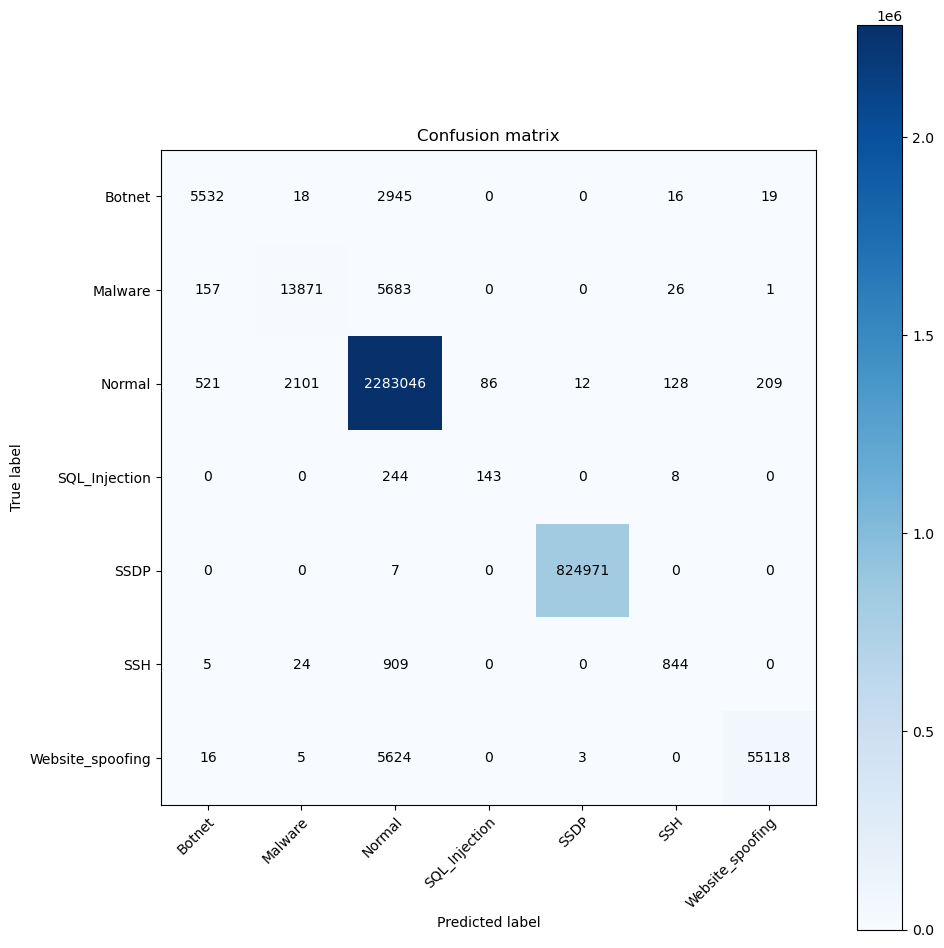
\includegraphics[width=0.85\textwidth]{Appendices/NN Confusion Matrix 3-04-23.png}
%    \caption{RF Confusion Matrix}
%    \label{fig:rf_confusion_matrix}
%\end{figure}

 \newpage

\subsubsection{XGBoost}
\label{sec:xgboost}

As discussed earlier, the XGBoost classifier was first trained with default parameters across a range of subsets of data before attempting to optimise parameters using 10 Fold Stratified Cross Validation to verify results across the training set. Finally, the test set (30\% of the overall data) was used to evaluate each model on a series of unseen data.

In the initial experiments, even without tuning parameters, the models achieved a high performance across all metrics. Table \ref{tab:xgb-scv-metrics} summarises the average metrics with 10 Fold Stratified Cross-Validation and Table \ref{tab:xgb-test-metrics} shows the metrics across the 30\% test set. Due to the numerous models created during experimentation, only the most notable models are included in the tables.


\begin{table}[h]
\centering
\caption{XGBoost S-CV Metrics}
\label{tab:xgb-scv-metrics}
\begin{tabular}{|l|l|l|l|l|l|l|l|}
\hline
\textbf{Model ID} & \textbf{Dataset} & \textbf{AUC} & \textbf{F1} & \textbf{Precision} & \textbf{Recall} & \textbf{Accuracy}  \\ \hline
1006 & 100\% & 99.99 & 99.64 & 99.64 & 99.64 & 99.64 \\ \hline
1008 & 100\% & 99.99 & 99.64 & 99.64 & 99.65 & 99.65 \\ \hline
1010 & 100\% & 100.00 & 99.65 & 99.65 & 99.66 & 99.66 \\ \hline
1011 & 100\% & 100.00 & 99.64 & 99.64 & 99.65 & 99.65 \\ \hline
\end{tabular}
\end{table}



\begin{table}[h]
\centering
\caption{XGBoost Test Metrics}
\label{tab:xgb-test-metrics}
\begin{tabular}{|l|l|l|l|l|l|l|l|}
\hline
\textbf{Model ID} & \textbf{Dataset} & \textbf{AUC} & \textbf{F1} & \textbf{Precision} & \textbf{Recall} & \textbf{Accuracy}  \\ \hline
1000 & 60\% & 99.99 & 99.63 & 99.64 & 99.64 & 99.64 \\ \hline
1001 & 80\% & 99.99 & 99.64 & 99.65 & 99.65 & 99.65 \\ \hline
1002 & 80\% & 99.99 & 99.64 & 99.64 & 99.64 & 99.64 \\ \hline
1003 & 80\% & 99.99 & 99.64 & 99.64 & 99.64 & 99.64 \\ \hline
1005 & 80\% & 99.99 & 99.64 & 99.65 & 99.65 & 99.65 \\ \hline
1006 & 100\% & 99.99 & 99.65 & 99.65 & 99.65 & 99.65 \\ \hline
1008 & 100\% & 99.99 & 99.65 & 99.65 & 99.65 & 99.65 \\ \hline
1010 & 100\% & 99.99 & 99.65 & 99.65 & 99.66 & 99.66 \\ \hline
1011 & 100\% & 99.99 & 99.65 & 99.65 & 99.65 & 99.65 \\ \hline
\end{tabular}
\end{table}


%\begin{table}[h]
%\centering
%\caption{XGB Model Metrics}
%\label{tab:xgb-metrics}
%\begin{tabular}{|l|l|l|l|l|l|l|l|}
%\hline
%\textbf{Model} & \textbf{Device} & \textbf{Dataset} & \textbf{AUC} & \textbf{Accuracy} & \textbf{Precision} & \textbf{Recall} & \textbf{F1}  \\ \hline
%Base & M2 & 80\% & ? & 99.7 & 95.5 & 88.2 & 91.5 \\ \hline
%Base & M2 & 100\% & ? & ? & ? & ? & ? \\ \hline
%Base & VM & 60\% & ? & 99.6 & 95.0 & 88.4 & 91.4 \\ \hline
%Base & VM & 80\% & 1.00 & 99.6 & 94.9 & 87.8 & 91.0 \\ \hline
%Base & VM & 100\% & ? & 99.7 & 99.7 & 99.7 & 99.6 \\ \hline
%Optimised & VM & 80\% & 1.00 & 99.6 & 99.6 & 99.6 & 99.6 \\ \hline
%Optimised & VM & 100\% & 1.00 & 99.7 & 99.6 & 99.7 & 99.6 \\ \hline
%RGS & VM & 100\% & 99.99 & 99.66 & 99.65 & 99.66 & 99.65 \\ \hline
%\end{tabular}
%\end{table}

\subsubsection*{Randomised GridSearch}

An attempt was made to utilise GridSearchCV for parameter optimization; significant setbacks were encountered in achieving a successful execution due to numerous errors, system crashes, and exceptionally high grid search time. In light of the difficulties faced with GridSearchCV, RandomizedSearchCV was utilised instead, This decision was justified by several factors:

RandomizedSearchCV uses a subset of parameter combinations sampled from a defined grid. This approach heavily reduces the computational power required compared to the exhaustive search needed for GridSearchCV. Moreover, RandomizedSearchCV enables striking a balance between computational resources and search comprehensiveness by defining the number of iterations to evaluate. See Listing \ref{lst:param_grid_xgb} for the parameter grid used.

\medskip

\begin{lstlisting}[language=Python, caption={Grid Search Parameters For XGBoost}, label= lst:param_grid_xgb]
param_grid = {
    'learning_rate': [0.01, 0.1, 0.3],
    'max_depth': [3, 6, 9],
    'min_child_weight': [1, 3, 5],
    'gamma': [0, 0.1, 0.2],
    'subsample': [0.5, 0.7, 0.9],
    'colsample_bytree': [0.5, 0.7, 0.9],
    'n_estimators': [100, 200]
}
\end{lstlisting}

\textbf{Best Found Parameters}
\medskip

Using the best-found parameters from the RandomizedSearchCV, a new model was created, referenced above as ID 1010. Table \ref{tab:xg_rgs_parameters} highlights the optimal parameters found.

\begin{table}[h]
\captionsetup{justification=centering} 
\centering
\caption{XGBoost RGS Parameters}
\begin{tabular}{ll}
\hline
\textbf{Parameter} & \textbf{Value} \\ \hline
Early Stopping & 10 \\
Evaluation Metric & merror \\
Learning Rate & 0.3 \\
Max Depth & 9 \\
Min Child Weight & 3 \\
Gamma & 0 \\
Subsamples & 0.9 \\
Colsample By Tree & 0.7 \\
N Estimators & 200 \\ \hline
\end{tabular}
\label{tab:xg_rgs_parameters}
\end{table}


\textbf{Optimised Model}
\medskip

A new model was created with the best-found parameters, this is referred to as the 'Optimised Model'/(ID 1010) in this section. The model performed very well, with an average AUC of 99.99 on the training data and 99.98 on the test data. The F1 score is 99.65 on the test set indicating the model has a high proportion of correct predictions, balancing both precision and recall well. The confusion matrix verifies this and shows the model to perform well for most classes, especially Normal, SDDP and Web Spoofing with almost perfect precision and recall. However, there are a few misclassifications for 'Botnet', 'Malware' and 'SSH'. The model struggled and occasionally misclassified Normal traffic as malicious, but performed well in the SQL Injection class, especially given the small number of samples. The Cross-validation and test set results are similar and indicate the model is not overfitting and generalising well to new data. Refer to \ref{fig:xgb_optimised_fi}, \ref{fig:xgb_optimised_cm} and \ref{tab:optimised_xgboost} for metrics.

Using the total number of instances of each class, the misclassification report can be calculated for each and is shown accordingly:

\begin{itemize}
	\item Botnet: 4208 / 17060 = {\color{red} 25\%}
	\item Malware: 7161 / 39476 = 18\%
	\item Normal: 6365 / 4572206 = 0.0013\%
	\item SQL: 89 / 789 = 11\%
	\item SSDP: 0 / 1649955 = {\color{mygreen} 0\%}
	\item SSH: 771 / 3565 = 21\%
	\item WebSpoof: 3046 / 121533 = 2.5\%
\end{itemize}


\begin{figure}[H]
\centering
\caption{Optimised XGBoost Model FI}
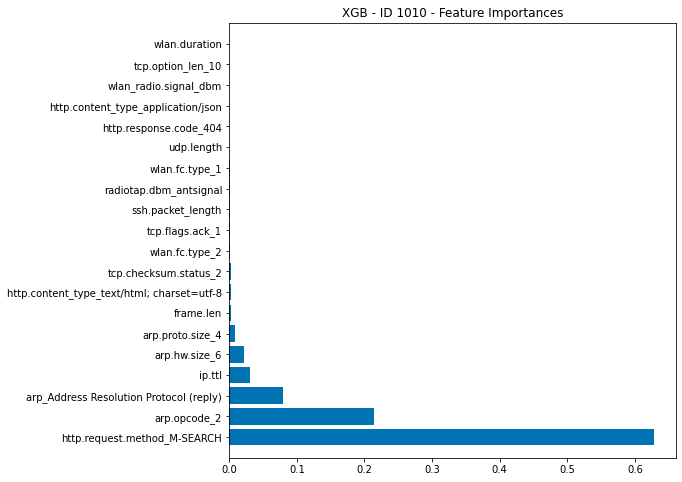
\includegraphics[width=\textwidth]{Appendices/Images/XGB/xgb_1010_fi.png}
\label{fig:xgb_optimised_fi}
\end{figure}

\clearpage
\begin{table}[hp]
  \centering
  \caption{Optimised XGBoost Classification Report}
  \label{tab:optimised_xgboost}
    \begin{tabular}{lcccc}
    \toprule
    Class & Precision & Recall & F1-Score & Support \\
    \midrule
    Botnet & 0.96 & {\color{red}\bfseries 0.75} & {\color{red}\bfseries 0.84} & 17060 \\
    Malware & {\color{red}\bfseries 0.89} & 0.82 & 0.85 & 39476 \\
    Normal & 1.00 & 1.00 & 1.00 & 4572206 \\
    SQL Injection & 0.94 & 0.89 & 0.91 & 789 \\
    SSDP & 1.00 & 1.00 & 1.00 & 1649955 \\
    SSH & 0.92 & 0.78 & 0.85 & 3565 \\
    Website Spoofing & 0.99 & 0.97 & 0.98 & 121533 \\
    \midrule
    Accuracy & & & 1.00 & 6404584 \\
    Macro Avg & 0.96 & 0.89 & 0.92 & 6404584 \\
    Weighted Avg & 1.00 & 1.00 & 1.00 & 6404584 \\
    \bottomrule
    \end{tabular}
\end{table}

\begin{figure}[H]
\centering
\caption{Optimised XGBoost Model CM}
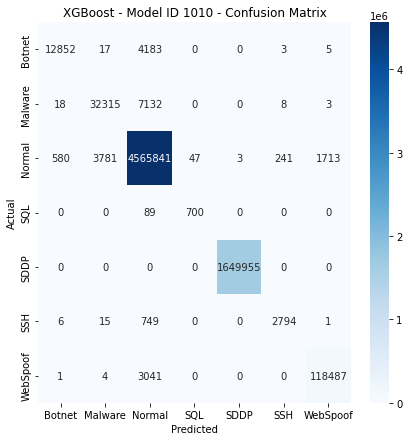
\includegraphics[width=0.9\textwidth]{Appendices/Images/XGB/xgb_1010_cm.png}
\label{fig:xgb_optimised_cm}
\end{figure}



%
%\begin{table}[h]
%\centering
%\caption{XGBoost Evaluation Metrics}
%\label{tab:xgb-eval-metrics}
%\begin{tabular}{|l|l|l|l|l|l|l|l|}
%\hline
%\textbf{Model} & \textbf{Device} & \textbf{Size} & \textbf{AUC} & \textbf{F1} & \textbf{Precision} & \textbf{Recall} & \textbf{Accuracy} \\ \hline
%Stock & M2 & 80\% & ? & 91.5 & 95.5 & 88.2 & 99.7 \\ \hline
%Stock & M2 & 100\% & 99.99 & 99.65 & 99.65 & 99.65 & 99.65 \\ \hline
%Stock & VM & 60\% & ? & 91.4 & 95.0 & 88.4 & 99.6 \\ \hline
%Stock & VM & 80\% & 1.00 & 91.0 & 94.9 & 87.8 & 99.6 \\ \hline
%Stock & VM & 100\% & ? & 99.6 & 99.7 & 99.7 & 99.7 \\ \hline
%Optimised & VM & 80\% & 1.00 & 99.6 & 99.6 & 99.6 & 99.6 \\ \hline
%Optimised & VM & 100\% & 1.00 & 99.6 & 99.6 & 99.7 & 99.7 \\ \hline
%RGS & VM & 100\% & 99.99 & 99.65 & 99.65 & 99.66 & 99.66 \\ \hline
%\end{tabular}
%\end{table}


\subsubsection{KNN Classifier}

During initial experimentation, KNN took over 22 hours to predict on our test data set after training - Figure \ref{fig:knn_train}. Additionally, utilising the second VM machine, KNN took over 28 hours to predict the test set of data, and subsequently crashed the system multiple times before we could gather results or evidence. KNN's algorithm means it does not build and store a model during training but rather stores them in memory. As a result, when we predict on the test set we encounter a high computational complexity task as KNN searches for the K-nearest neighbour from our training set. As we have a relatively large amount of features, this further increases the computational power required for these tasks. This was deemed too long for real-world applications where detecting network attacks would be time-sensitive. As network attacks can occur quickly, an IDS using ML algorithms need to have a quick response to detecting these attacks.

Despite the advantages of KNN, such as being easy to implement and interpret, the prioritisation of speed and accuracy in this work led to the ultimate decision not to continue with this classifier. Consequently, the results for this classifier remain inconclusive.

\medskip

\begin{figure}[h]
\caption{Training Time for KNN Classifier}
\label{fig:knn_train}
\centering
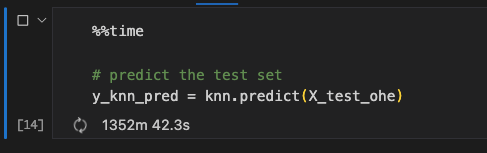
\includegraphics[width=\textwidth]{Appendices/Images/knn_predict-2023-04-15.png}
\end{figure}
\subsection{Neural Networks}
\label{sec: Neural Networks}

\subsubsection{Multi-Layer Perceptron (MLP)}
\label{sec: MLP Neural Network v1}

As part of the neural network experiments, Multilayered Perceptron models were created and tested through an exploratory process. It should be noted a wide range of MLP models was explored, the selection presented in the results section is a curated list, chosen for performance or notability. All models evaluated and their corresponding code can be found within the codebase. Table \ref{tab:mlp-models-1} and \ref{tab:mlp-models-2} details the set of parameters used for each notable MLP model.  

Experimentation began with a 3 hidden layered MLP model consisting of 128, 64 and 32 neurons across the different subsets of data to gauge a rough estimate of the model's performance through varying levels of data. As such, cross-validation was not utilised. Models 0-3 consist of the same parameters tested across the 60 and 80\% datasets, metrics were high, however, the models struggled to predict minority classes and resulted in low recall and F1-Scores. Performance when increasing the size of the dataset did improve the performance and can be attributed to the fact the larger dataset provided more samples of the minority class to be trained on. With this information, further models were created with increased batch sizes and epochs to train for longer.

\subsubsection*{Overfitting}

A key aspect when training the MLP models was to prevent overfitting. To help mitigate this, techniques such as Early Stopping and Dropout were used in the majority of the models. Early Stopping was used during SCV, the training process monitors the validation AUC loss for signs of overfitting (e.g. when the model starts to learn the data and not generalising). Once the validation loss started to degrade over two defined epochs, the model would stop training. Dropout is a regularisation method that randomly sets 0.2 of the input neurons to 0. Dropout layers were used in the network architecture.

 
\subsubsection*{Thresholds}
Towards the latter stages of experimentation, an attempt was made to further enhance the performance of the models on the misclassified classes. The individual class weightings were adjusted using the thresholds of each class. The aim was to identify the optimal threshold level between 0-1 that would maximise the F1 score for that class. A systematic approach was followed to adjust the value in the class and evaluate the confusion matrices for changes in predictions.
 
 
\subsubsection*{Activator}
Due to the nature of the problem (multi-class classification), applying existing knowledge and experience, the softmax activator was chosen for the output layer. It provides an easy-to-interpret output of the model as a list of probabilities for each class and uses the highest probability as the predicted class.

\subsubsection*{Tuning}

The device used to train and the experiment was the M2 Mac Mini, experiments conducted on the VM were found to be slower and would frequently cause crashes, even when utilising the dedicated GPU. As such, the hardware and time constraints restricted the level of tuning and parameter searching that could be performed. Techniques such as GridSearchCV and RandomisedSearchCV were not feasible when combined with 10 Fold S-CV. 

\medskip
Due to the complexity and computational demands of running machine learning models, practical limitations such as time constraints result in fewer tested models than desired. After conducting a vast amount of experiments and achieving high-performance results, the decision was made to conclude further model experimentation. 
 
\medskip
\begin{table}[H]
\centering
\caption{MLP Model Parameters Part 1}
\label{tab:mlp-models-1}
\begin{tabular}{llll}
\hline
Parameter & Model 0-3 & Model 4 & Model 5 \\ \hline
Asctivator: & ReLU & ReLU & ReLU \\
Output Activator: & Softmax & Softmax & Softmax \\
Initialiser: & he\_uniform & he\_uniform & he\_uniform \\
Optimiser: & Adam & Adam & SGD \\
Momentum: & N/A & N/A & N/A \\
Early Stopping: & N/A & 2 & 2 \\
Dropout: & 0.2 & 0.2 & 0.2 \\
Learning Rate: & 0.001 & 0.001 & 0.01 \\
Loss: & CC & CC & CC \\
Batch Norm: & True & True & True \\
Hidden Layers: & 3 & 3 & 4 \\
Nodes per Layer: & 128/64/32 & 128/64/32 & 256/128/64/32 \\
Batch Size: & 180 & 200 & 132 \\
Epochs: & 15 & 20 & 20 \\ \hline
\end{tabular}
\end{table}

\begin{table}[H]
\centering
\caption{MLP Model Parameters Pt2}
\label{tab:mlp-models-2}
\begin{tabular}{lll}
\hline
Parameter         & Model 6       & Model 7         \\ \hline
Activator:        & LeakyReLU     & ReLU            \\
Output Activator: & Softmax       & Softmax         \\
Initialiser:      & he\_uniform   & -               \\
Optimiser:        & Adam          & SGD             \\
Momentum:         & N/A           & 0.9             \\
Early Stopping:   & 2             & 2               \\
Dropout:          & 0.2           & 0.25*3/0.2*2    \\
Learning Rate:    & 0.01          & 0.01            \\
Loss:             & CC            & CC              \\
Batch Norm:       & True          & True            \\
Hidden Layers:    & 4             & 5               \\
Nodes per Layer:  & 256/128/64/32 & 100/80/60/40/20 \\
Batch Size:       & 132           & 170             \\
Epochs:           & 20            & 20              \\ \hline
\end{tabular}
\end{table}

%Table \ref{tab:seq_nn} specifies the parameter values for a multi-layered feed-forward neural network model, consisting of one input layer (128 neurons) and one hidden layer (64 neurons) using the ReLu activator function. The output layer has a subsequent 7 neurons corresponding to the 7 different output classes, using a soft-max activation function to produce the class probabilities. See Appendix \ref{appx: MLP NN v1} for the full code.
%



%!TEX root =  ../Report.tex

\section{Analysis Of Results}
 \label{sec: Analysis Of Results}

% TODO Summarise the Results of each model here and talk about the best model here. 

In this section, the performance of the machine learning models on the test set is analysed and discussed. The models are evaluated using the metrics discussed previously, such as F1-Score, Area Under Curve (AUC), Precision, Recall and Accuracy. The best-performing models and algorithms are identified and interpreted. Finally, limitations and challenges faced in the analysis are discussed and addressed and areas of improvement for future work are suggested.


\subsection{Random Forest}

Six notable models were trained during experimentation with the Random Forest Classifier with a series of parameters and values. Tables \ref{tab:rf-scv-metrics} and \ref{tab:rf-test-metrics} show the S-CV and Test metrics for AUC, F1, Precision, Recall and Accuracy. Each model's individual metrics, classification report, confusion matrix and feature importances can be found in Appendix \ref{appx:Random Forest}.
 
\begin{table}[H]
\centering
\caption{RF S-CV Mean Metrics}
\label{tab:rf-scv-metrics}
\begin{tabular}{|l|l|l|l|l|l|l|}
\hline
\textbf{Model ID} & \textbf{Size} & \textbf{AUC} & \textbf{F1} & \textbf{Precision} & \textbf{Recall} & \textbf{Accuracy}  \\ \hline
1 & 100\% & 99.99 & 99.66 & 99.66 & 99.68 & 99.67 \\ \hline
3 & 100\% & 99.99 & 99.66 & 99.66 & 	99.67 &	99.67 \\ \hline
4 & 100\% & 99.95 & 95.23 &	98.50 &	92.96 &	92.96 \\ \hline
5 & 100\% & 99.87 &	91.53 &	98.42 &	86.65 &	86.65 \\ \hline
\end{tabular}
\end{table}

\begin{table}[h]
\centering
\caption{RF Test Metrics}
\label{tab:rf-test-metrics}
\begin{tabular}{|l|l|l|l|l|l|l|}
\hline
\textbf{Model ID} & \textbf{Size} & \textbf{AUC} & \textbf{F1} & \textbf{Precision} & \textbf{Recall} & \textbf{Accuracy}  \\ \hline
0 & 80\% & 99.99 & 99.66 & 99.66 & 99.67 & 99.67 \\ \hline
1 & 100\% & 99.99 & 99.66 & 99.66 & 99.67 & 99.67 \\ \hline
2 & 100\% & 99.99 & 99.66 & 99.66 & 99.67 & 99.67 \\ \hline
3 & 100\% & 99.99 & 99.66 & 99.66 & 99.67 & 99.67 \\ \hline
4 & 100\% & 99.95 & 98.48 &	92.54 & 94.97 &	92.54 \\ \hline
5 & 100\% & 99.86 & 91.17 & 98.48 & 86.01 & 86.01 \\ \hline
\end{tabular}
\end{table}

\textbf{Models 0-2}

\smallskip
Models 0-2 all used the default parameters for the RandomForestClassifier, and therefore share similar results across metrics.

Despite model 0 being trained on an 80\% subset of the data, its performance was similar to models 1 and 2, achieving test metrics of AUC: 99.99\%, F1: 99.66\%, Precision: 99.66\%, Recall: 99.67\% and Accuracy of 99.67\%. The model achieved a perfect score for SDDP, with only seven misclassifications. Examining the classification report shows low recall for less represented classes such as Botnet and SSH, with recalls of 0.77 and 0.78, this is further verified by the confusion matrix. 
Models 1 and 2 were trained on the entire dataset, with the exception that model 1 was trained with 10 Fold Stratified Cross Validation meanwhile model 2 was not. Interestingly despite the change in dataset sizes, the models appear to perform nearly identically with the same consistently high metrics across both Cross Validation and Testing, suggesting the models are not overfitting. As seen in model 0, the classification reports and confusion matrix shares similar performances, with model 1 and 2 having a smaller number of misclassifications i.e. from 7 false positives to 2 on the SDDP class. This may indicate that despite adding more data to training, the RandomForestClassifier was unable to learn from the extra information which leads to diminishing returns for this specific problem. 
 
\medskip
\textbf{Class Weight}

During experimentation, models 3 and 5 share almost identical parameters except for the parameter: \textit{class\_weight}. The Class Weight parameter allows for the classifier to handle imbalanced datasets, its default value is \textit{None}, meaning the model treats every class as equal during the training process. Alternatively, when set to \textit{'balanced'}, the model assigns high weights that are inversely proportional to the class frequencies \parencite{scikit-learn}. Model 5's class weight is set to \textit{balanced} compared to \textit{None}. When evaluating the results, model 3 supersedes model 5 across almost every metric, with a higher F1, precision, recall and accuracy score with the following percentage decrease per metric: AUC: 0.12\%, F1: 8.18\%, Precision: 1.24\%, Recall: 12.99\%, Accuracy: 12.99\%. In terms of classification, Model 3 struggled with some of the minority classes such as Botnet, SSH and Malware, on the other hand, model 5 had a higher recall for these classes, but suffered at the cost of a reduced precision for the Normal class. This suggests that even though higher weighting is given to the majority class, it does not necessarily lead to a better model in this scenario.

It was proposed this was due to Random Forest's majority voting decision factor, so although minority classes may have had a higher weighting, the class that has fundamentally more samples will have more trees \textit{'voting'} for that class.

% TODO talk about the results of the models with respect to the test set and metrics.


\medskip
\textbf{Feature Importance}

For all the models, the feature importance of each model was collected and inferred. The feature importance provides a score for each metric and highlights how important each feature was to the creation of the random forest models. In particular, the top five features were as follows:

\begin{itemize}
	\item \textit{ip.ttl} Appeared in the top five for all models and was the number one feature for models 1,2,3 and 5. The TTL value in the dataset may be containing a series of patterns relating to the different network attacks.
	\item \textit{http.request.method\_M-SEARCH} also appeared as one of the top features across a few of the models and was the number one feature in model 0. 
	\item \textit{udp.length} This feature appeared in the top three features except for model 5.
  	\item \textit{radiotap.dbm\_antsignal} was in the top five features for all models, gaining number one importance in model 5.
	\item \textit{wlan\_radio.duration} was also prevalent in the top five features across most models.
	\item \textit{frame.len} was also prevalent in the top five features across most models.
	\item \textit{wlan\_radio.signal\_dbm} and \textit{wlan\_radio.duration} gained an increase in performance across model 5, this could be the effects of adjusting the class weighting to \textit{balanced} for the model.
\end{itemize}


% TODO Talk about the feature importance diagrams and how they relate to the problem at hand.
\medskip
Overall the Random Forest models showed strong performances across the classes, however, due to the imbalanced nature of the dataset, it may have hidden the weaknesses within the minority classes (e.g. SQL Injection \& SSH). Iterative and exploratory experimentation showed that the default parameters achieved superior results compared to the other models. Future work should focus on using GridSearchCV and RandomisedSearchCV to provide more advanced parameter tuning. Moreover, further emphasis can be placed on the minority classes to help lower the number of false positives.


% !TEX root =  ../Report.tex

\section{Conclusion}
\label{sec: Conclusion}

% \lipsum[7]

\subsection{Summary Of Findings}

Summarize the main findings of your research, including the performance of your machine learning models, insights gained from the analysis, and any limitations or areas for future work.

\subsection{Implications}

 Discuss the implications of your research for the field of machine learning and for the specific problem you addressed. This could include discussing how your research advances the state-of-the-art, how it could be applied in practice, or how it could inform future research.
 
\subsection{Contributions}

Discuss the contributions of your research to the field of machine learning. This could include discussing how your research fills a gap in the literature, how it provides new insights into the problem you addressed, or how it advances the methodology used in the field.

\subsection{Limitations}

Discuss the limitations of your research and potential sources of error. Explain how these limitations could impact the generalizability of your findings and suggest ways to address these limitations in future research.

\subsection{Future Work}

Discuss potential future work that could be done to build on your research and improve the performance of machine learning models in the specific problem you addressed and in the field more broadly.

% !TEX root =  ../Report.tex

%\section{Chapter 7}
%\label{Sec: Chapter 7}

%\lipsum[8]


%!TEX root =  ../Report.tex

%\section{Conclusions}
%\label{sec:Chapter 8}

%\lipsum[9]



% !TEX root =  ../Report.tex
%\section{Making a reference}
% \label{sec: Reference}

% \noindent In this chapter we shall do a reference to an entry in the bibliography, \texttt{bibliography.bib}. \\

% What we know of the invention of the flux capacitor is that Dr. Emmett Brown thought of this when hanging a clock in the bathroom. He was standing on his porcelain sink and slipped because it was wet, the resulting hit on the head was apparently a cause to this invention \cite{example}.\\

% The corresponding sketch made on this day has been attached in appendix \ref{appx: Flux Sketch}.


%Keep adding folders as to your desires

% \bibliographystyle{abbrv}
%\nocite{*}
\printbibliography[heading=bibintoc,title={Bibliography}]

\begin{appendices}
\addcontentsline{toc}{section}{Appendices}


%\section{The Flux Sketch}
%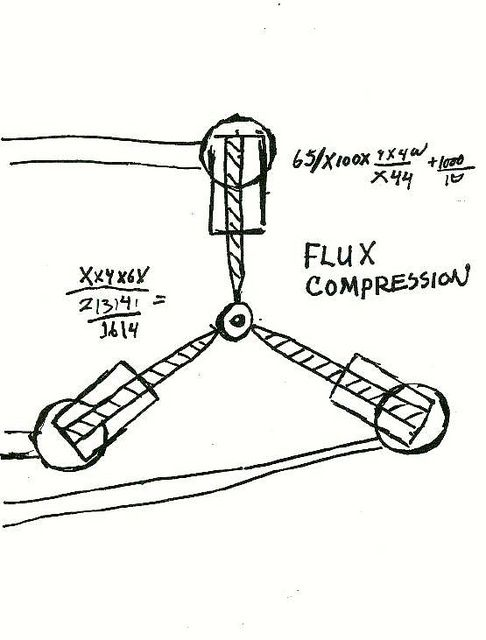
\includegraphics[width=\textwidth]{Report/Appendices/flux_sketch.jpg}
%\label{appx: Flux Sketch}


\section{Data-set Manipulation}

\subsection{CSV Combiner Script}
\label{appx: CSV Combiner Script}
\begin{lstlisting}
#!/bin/bash

# Input Directory
input_dir="../Malware"

cd "$input_dir"

# Set the output file name
output_file="combined.csv"

# Check if the output file already exists and delete it
if [ -f "$output_file" ]; then
  rm "$output_file"
fi

# Print a status message
echo "Combining files..."

# Loop through all the files that match the pattern reduced_*.csv
for file in $(ls *.csv | sort -V)
do
  # Check if the file exists
  if [ -f "$file" ]; then
    # Print a status message
    echo "Combining $file..."

    # If this is the first file, copy the header to the output file
    if [ ! -f "$output_file" ]; then
      head -n 1 "$file" > "$output_file"
    fi

    # Append all the rows except the header to the output file
    tail -n +2 "$file" >> "$output_file"
  fi
done

# Print a status message
echo "Done."
\end{lstlisting}

\newpage
\subsection{Feature Extraction \& Reduction}
\label{appx: Feature Extraction}

\begin{lstlisting}
# Define the columns you want to keep
cols_to_use = ['frame.len', 'radiotap.dbm_antsignal', 'radiotap.length', 'wlan.duration',
                   'wlan_radio.duration', 'wlan_radio.signal_dbm', 'radiotap.present.tsft',
                   'wlan.fc.type', 'wlan.fc.subtype', 'wlan.fc.ds', 'wlan.fc.frag',
                   'wlan.fc.moredata', 'wlan.fc.protected', 'wlan.fc.pwrmgt', 'wlan.fc.retry',
                   'wlan_radio.phy', 'udp.length', 'ip.ttl', 'arp', 'arp.proto.type',
                   'arp.hw.size', 'arp.proto.size', 'arp.hw.type', 'arp.opcode',
                   'tcp.analysis', 'tcp.analysis.retransmission', 'tcp.option_len',
                   'tcp.checksum.status', 'tcp.flags.ack', 'tcp.flags.fin', 'tcp.flags.push',
                   'tcp.flags.reset', 'tcp.flags.syn', 'dns', 'dns.count.queries', 'dns.count.answers',
                   'dns.resp.len', 'dns.resp.ttl', 'http.request.method', 'http.response.code',
                   'http.content_type', 'ssh.message_code', 'ssh.packet_length', 'nbns',
                   'nbss.length', 'nbss.type', 'ldap', 'smb2.cmd', 'smb.flags.response',
                   'smb.access.generic_read', 'smb.access.generic_write', 'smb.access.generic_execute','Label']

# Define the chunk size you want to read in each iteration
batch_size = 1000000

# Initialize an empty dataframe to hold the combined results
combined_df = pd.DataFrame()

# Iterate through the file in batches
for chunk in pd.read_csv('botnet_combined.csv', chunksize=batch_size, usecols=cols_to_use, low_memory=False):
    
    # Combine the processed chunk with previous chunks
    combined_df = pd.concat([combined_df, chunk])
\end{lstlisting}

\newpage
\begin{lstlisting}
# Drop all missing rows that contain only nan values
combined_df = combined_df.dropna(how='all')

# Drop all rows with missing values in Label Column
combined_df = combined_df.dropna(subset=['Label'])

# Fill NAs with zeros
# Change nan values to 0
combined_df = combined_df.fillna(0)
\end{lstlisting}

\begin{lstlisting}
# Duplicate the dataframe
df = combined_df.copy()

# Regex to keep only the first value e.g 
# -100-100-10 becomes -100,   123-456-1 becomes 123, -10-2 becomes-10, 81-63-63 becomes 81
def seperated_values(x):
    x = str(x)
    match = re.match(r'^(-?\d+).*$', x)
    if match:
        return match.group(1)
    else:
        return x

# Go through all columns and change seperate values into just one value
for column in df.columns:
    df[column] = df[column].apply(seperated_values)
    print('Processing', column)
print('Done')

# Find Rows that contain values such as Oct-26, Oct-18, Feb-10 etc.. as these appear to be invalid and we will drop these rows.
regex = r"\b(?:\d{2}|(?:Jan|Feb|Mar|Apr|May|Jun|Jul|Aug|Sep|Oct|Nov|Dec))-(?:\d{2}|(?:Jan|Feb|Mar|Apr|May|Jun|Jul|Aug|Sep|Oct|Nov|Dec))\b"

# Use str.match method to apply the regex pattern to the column
mask = df['tcp.option_len'].astype(str).str.match(regex).fillna(False)
df = df[~mask]

mask = df['dns.resp.ttl'].astype(str).str.match(regex).fillna(False)
df = df[~mask]

mask = df['ip.ttl'].astype(str).str.match(regex).fillna(False)
df = df[~mask]

mask = df['smb2.cmd'].astype(str).str.match(regex).fillna(False)
df = df[~mask]

df.to_csv('Botnet_Reduced.csv', index=False)    

\end{lstlisting}

\newpage

\section{Conda Environments}
\label{appx: Conda_Env}

\subsection{Neural Networks - Apple Silicon}

\begin{lstlisting}
conda create -n nn-env python=3.9
conda activate nn-env
conda install -c apple tensorflow-deps
conda install -c conda-forge -y pandas jupyter
pip install tensorflow-macos==2.10
pip install numpy, matplotlib, scikit-learn, scipy, seaborn
\end{lstlisting}

\subsection{Classifiers}

\begin{lstlisting}
# Conda environment used for Random Forest, XGBoost and K-NN.

conda create -n ml-env python=3.9
conda activate ml-env
conda install -c conda-forge -y pandas jupyter
pip install numpy, matplotlib, scikit-learn, scipy, seaborn, xgboost
\end{lstlisting}

\newpage

\section{Data Preprocessing}
\label{appx:Data Processing}

\subsection{MinMax Scaling}
\label{appx:Scaling}

\begin{lstlisting}
# Define the scaler
scaler = MinMaxScaler()

# Fit the scaler to the following columns we define
scale_cols = [
        'frame.len',
        'radiotap.dbm_antsignal', 
        'radiotap.length', 
        'wlan.duration', 
        'wlan_radio.duration', 
        'wlan_radio.signal_dbm',
        'ip.ttl', 
        'udp.length', 
        'nbss.length',
        'dns.count.answers', 
        'dns.count.queries',
        'dns.resp.ttl',
        'ssh.packet_length']
        
# Fit the X_train and X_test
X_train[scale_cols] = scaler.fit_transform(X_train[scale_cols])
X_test[scale_cols] = scaler.transform(X_test[scale_cols])
\end{lstlisting}

\subsection{OHE Encoding}
\label{appx:OHE Encoding}
\begin{lstlisting}
cols_to_encode = [col for col in X_train.columns if col not in scale_cols]
X_all = pd.concat([X_train, X_test], axis=0)

X_all_ohe = pd.get_dummies(X_all, columns=cols_to_encode, drop_first=True, dtype=np.uint8)

# split back into train and test sets
X_train_ohe = X_all_ohe[:len(X_train)]
X_test_ohe = X_all_ohe[len(X_train):]
\end{lstlisting}

\newpage
\subsection{Label Encoding}
\label{appx:Label Encoding}
\begin{lstlisting}
    # Use Label Encoder to encode the target variable
le = LabelEncoder()

label_encoder = le.fit(y_train)
y_train_encoded = label_encoder.transform(y_train)
\end{lstlisting}

\subsection{Loading Dataset}
\label{appx:Loading Dataset}
\begin{lstlisting}
chunk_size = 1000000
dtype_opt = {
    'frame.len': 'int64',
    'radiotap.dbm_antsignal': 'int64',
    'radiotap.length': 'int64',
    'radiotap.present.tsft': 'int64',
    'wlan.duration': 'int64',
    'wlan.fc.ds': 'int64',
    'wlan.fc.frag': 'int64',
    'wlan.fc.moredata': 'int64',
    'wlan.fc.protected': 'int64',
    'wlan.fc.pwrmgt': 'int64',
    'wlan.fc.type': 'int64',
    'wlan.fc.retry': 'int64',
    'wlan.fc.subtype': 'int64',
    'wlan_radio.duration': 'int64',
    'wlan_radio.signal_dbm': 'int64',
    'wlan_radio.phy': 'int64',
    'arp': 'object',
    'arp.hw.type': 'object',
    'arp.proto.type': 'int64',
    'arp.hw.size': 'int64',
    'arp.proto.size': 'int64',
    'arp.opcode': 'int64',
    'ip.ttl': 'int64',
    'tcp.analysis': 'int64',
    'tcp.analysis.retransmission': 'int64',
    'tcp.checksum.status': 'int64',
    'tcp.flags.syn': 'int64',
    'tcp.flags.ack': 'int64',
    'tcp.flags.fin': 'int64',
    'tcp.flags.push': 'int64',
    'tcp.flags.reset': 'int64',
    'tcp.option_len': 'int64',
    'udp.length': 'int64',
    'nbns': 'object',
    'nbss.length': 'int64',
    'ldap': 'object',
    'smb2.cmd': 'int64',
    'dns': 'object',
    'dns.count.answers': 'int64',
    'dns.count.queries': 'int64',
    'dns.resp.ttl': 'int64',
    'http.content_type': 'object',
    'http.request.method': 'object',
    'http.response.code': 'int64',
    'ssh.message_code': 'int64',
    'ssh.packet_length': 'int64'
}

# Read the data
print('Reading X...')
X = pd.DataFrame()
for chunk in pd.read_csv('X.csv', chunksize=chunk_size, usecols=dtype_opt.keys(), dtype=dtype_opt, low_memory=False):
    X = pd.concat([X, chunk])

print('Reading y...')
y = pd.DataFrame()
for chunk in pd.read_csv('y.csv', chunksize=chunk_size, usecols=['Label'], dtype='object', low_memory=False):
   y = pd.concat([y, chunk])

# Split the data into training and testing sets
print('Splitting the data...')
X_train, X_test, y_train, y_test = train_test_split(X, y, test_size=0.30, random_state=1234, stratify=y)
\end{lstlisting}

\newpage
\section{Classifiers}
\label{appx: Classifiers}

\subsection{Base K-Nearest Neighbor (KNN)}
\begin{lstlisting}
# Use KNN
from sklearn.neighbors import KNeighborsClassifier

k=5

# Create KNN classifier
knn = KNeighborsClassifier(n_neighbors=k, n_jobs=-1)

# Fit the model
knn.fit(X_train_ohe, y_train_encoded)

# predict the test set
y_knn_pred = knn.predict(X_test_ohe)

from sklearn.metrics import classification_report, roc_auc_score

# Get the classification report
report = classification_report(y_test_encoded, y_knn_pred)

print('Classification Report:\n', report)

# Get the all the metrics for the multi class classification

print('Accuracy: ', accuracy_score(y_test_encoded, y_knn_pred))
print('Precision: ', precision_score(y_test_encoded, y_knn_pred, average='macro'))
print('Recall: ', recall_score(y_test_encoded, y_knn_pred, average='macro'))
print('F1 Score: ', f1_score(y_test_encoded, y_knn_pred, average='macro'))

# Get the confusion matrix for multi-class and plot it
confusion = confusion_matrix(y_test, y_rf_pred)
print('Confusion Matrix\n')
print(confusion)

# Plot the confusion matrix for multi-class classification using seaborn
labels = ['Normal', 'SSDP', 'Website Spoofing', 'Malware', 'Botnet', 'SSH', 'SQL Injection']

plt.figure(figsize=(8, 8))
sns.heatmap(confusion, annot=True, fmt='d', cmap='Blues', xticklabels=labels, yticklabels=labels)
plt.title('Confusion Matrix')
plt.xlabel('Predicted')
plt.ylabel('Actual')
plt.show()

plt.figure(figsize=(10, 10))
feat_importances = pd.Series(rf.feature_importances_, index=X_train_ohe.columns)
feat_importances.nlargest(20).plot(kind='barh')
plt.show()
\end{lstlisting}

\subsection{XGBoost}

\subsubsection{Base XGBoost CF}
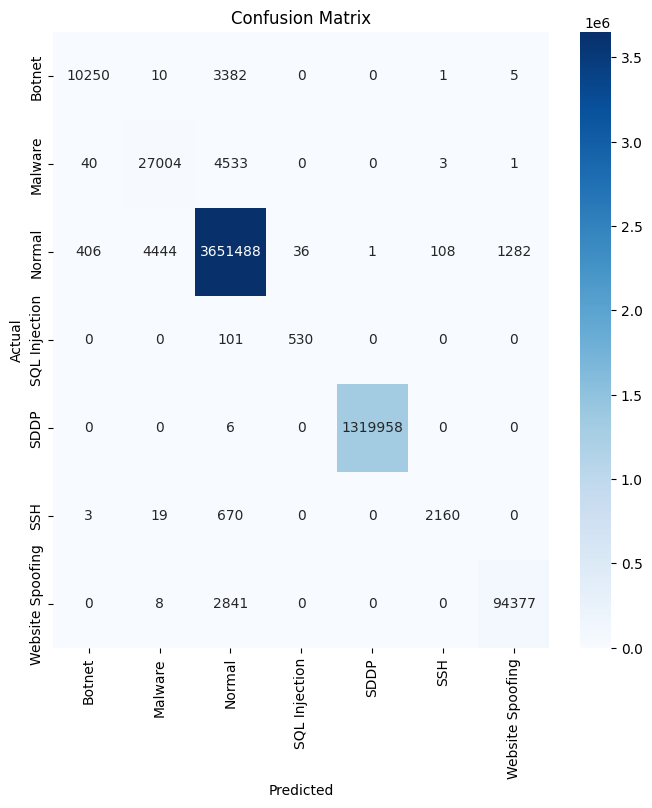
\includegraphics[width=\textwidth]{Appendices/Base_XGB_CF.png}
\newpage

\subsubsection{Base XGBoost Classification Report}
\begin{lstlisting}
                  precision    recall  f1-score   support

           0       0.96      0.75      0.84     13648
           1       0.86      0.86      0.86     31581
           2       1.00      1.00      1.00   3657765
           3       0.94      0.84      0.89       631
           4       1.00      1.00      1.00   1319964
           5       0.95      0.76      0.84      2852
           6       0.99      0.97      0.98     97226

    accuracy                           1.00   5123667
   macro avg       0.96      0.88      0.91   5123667
weighted avg       1.00      1.00      1.00   5123667
\end{lstlisting}

\newpage


\newpage



\section{Neural Networks}
\label{appx: Neural Networks}

\subsection{MLP NN v1}
\label{appx: MLP NN v1}

\begin{lstlisting}
# Create a sequential model
model = Sequential()
input_shape = (X_train_ohe.shape[1],)

# Add layers to the model
model.add(Dense(128, activation='relu', input_shape=input_shape))
model.add(Dense(64, activation='relu'))
model.add(Dense(7, activation='softmax'))

# Compile the model
model.compile(loss='categorical_crossentropy', optimizer='adam', metrics=['accuracy'])

# Train the model
model.fit(X_train_ohe, y_train_ohe, epochs=10, batch_size=32, validation_data=(X_test_ohe, y_test_ohe))

# Evaluate the model using test data
test_loss, test_acc = model.evaluate(X_test_ohe, y_test_ohe)

print('Test accuracy:', test_acc)
\end{lstlisting}

\subsubsection{MLP Neural Network}
\label{appx: MLP NN}

\begin{lstlisting}
from keras.models import Sequential
from keras.layers import Dense, Dropout, BatchNormalization
from keras.optimizers import SGD
from keras.initializers import he_uniform
from keras.metrics import AUC

# Define the number of classes
num_classes = 7

# Define the model architecture
model = Sequential()

# Add the input layer
model.add(Dense(100, input_shape=(X_train_ohe.shape[1],), activation='relu', kernel_initializer=he_uniform()))

# Add batch normalization
model.add(BatchNormalization())

# Add the first hidden layer
model.add(Dense(80, activation='relu', kernel_initializer=he_uniform()))
model.add(Dropout(0.25))
model.add(BatchNormalization())

# Add the second hidden layer
model.add(Dense(60, activation='relu', kernel_initializer=he_uniform()))
model.add(Dropout(0.2))
model.add(BatchNormalization())

# Add the third hidden layer
model.add(Dense(40, activation='relu', kernel_initializer=he_uniform()))
model.add(BatchNormalization())

# Add the fourth hidden layer
model.add(Dense(20, activation='relu', kernel_initializer=he_uniform()))
model.add(BatchNormalization())

# Add the output layer
model.add(Dense(num_classes, activation='softmax'))

# Define the optimizer
sgd = SGD(lr=0.01, momentum=0.9)

# Compile the model
model.compile(loss='categorical_crossentropy', optimizer=sgd, metrics=[AUC()])

# Train the model
batch_size = 170
epochs = 10
history = model.fit(X_train_ohe, y_train_ohe, batch_size=batch_size, epochs=epochs, validation_data=(X_test_ohe, y_test_ohe))

# Evaluate the model on your test data
test_loss, test_auc = model.evaluate(X_test_ohe, y_test_ohe)
\end{lstlisting}



\end{appendices}



\subsection{Evaluation Metrics}

A vital area of the work was deciding the use of specific metrics to evaluate the performance of the models. Metrics are essential to determine if models are under or over-fitting on the data and help to provide context into steps and modifications needed to improve the models' performances. 
As a multi-class classification problem, the primary focus was on the two main metrics of evaluation AUC and F1. Given the nature of the problem, it is essential to minimise false negatives and false positives, which represent misclassifying the attack on the network traffic as either a potential intrusion (false negative) or falsely marking regular traffic as malicious (false positives). By placing a strong emphasis on the F1 and AUC scores, this aims to provide a balanced measure of the model's performance.


\subsubsection*{AUC-ROC}

The Area Under the Receiver Operating Characteristic Curve (AUC-ROC) measures the ability of a model to distinguish between positive and negative classes correctly. AUC-ROC is also insensitive to class imbalances. Similarly, in the works carried out in \parencite{s22155633, pick_quality_over}, AUC was used as one of the primary evaluation metrics.

\medskip

This value is first calculated by plotting the Receiver Operating Characteristic (ROC) curve using the True Positive Rate (TPR) against the False Positive Rate (FPR) for each classification threshold. The TPR measures the proportions of positive values that were correctly classified. Similarly, the FPR is the proportion of negative values that are incorrectly classified as positive. The area under the curve (AUC) is calculated using the ROC curve. This value ranges between 0 and 1, where 0.5 represents, at best random guessing, and one corresponds to a perfect classifier.

\medskip

As the problem is multi-class, the AUC will be calculated by computing the one-vs-all metric for each class separately, i.e.,  calculated for each class individually, treating all samples for that class as positive and all others as negative. Then these scores are averaged to calculate a final AUC score.

\subsubsection*{F1}

The F1 score is a weighted average of both precision and recall. Precision is the fraction of correctly predicted positive instances out of all total predicted positive instances. The recall is the fraction of correctly predicted positive instances out of the total actual positive instances.

\subsubsection*{Equations for Precision, Recall \& F1} 

\begin{equation*} Precision = \frac{True\ Positive}{True\ Positive + False\ Positive} \end{equation*}

\begin{equation*} Recall = \frac{True\ Positive}{True\ Positive + False\ Negative} \end{equation*}

\begin{equation*}
F_1 = 2 \cdot \frac{\mathrm{Precision} \cdot \mathrm{Recall}}{\mathrm{Precision} + \mathrm{Recall}}
\end{equation*}

\subsubsection*{Micro, Macro and Weighted}

In regular binary classification, metrics such as F1, Precision, Recall and AUC can be calculated easily; however, for multi-class classification problems, a slightly different approach must be taken. In particular, there are three main methods:

\begin{itemize}
    \item Micro averaging uses the metric across all classes by counting the total true positives, false positives, and false negatives. This is the equivalent of using the accuracy, i.e., fails to consider class imbalances.
    \item Macro averaging calculates the metric in each class independently and then averages this for all classes, giving equal weight for all classes. It is typically used when all classes are equally important, regardless of class size or imbalance.
    \item Weighted averaging also calculates the metric for each class independently, but the average of the individual class scores is weighted with the number of samples in each class. It is used when performance across all classes is considered important, and the class imbalance needs to be considered.
\end{itemize}

Therefore, the weighted averaging method was chosen, leading to robust scores that consider both the number of samples within the class and its performance. It was observed that most previous works fail to mention the averaging method used for its evaluation metrics.

\subsubsection*{Classification Report}

In addition to viewing the averaged metrics across all classes, the classification report provides a comprehensive summary detailing the metrics for Precision, Recall, Accuracy and F1 across each class. This is important for understanding the underlying performance of the model, as underperforming classes can be identified, allowing guidance for tuning and modifications.

\subsubsection*{Confusion Matrix}

The Confusion Matrix is a table that displays the performance of a model by showing the number of true positives, false positives, true negatives and false negatives for each class. In other words, how accurate the classifier is on each class and how it tends to wrongly predict each class for another (confusion). By examining the confusion matrix, any specific classes that may require additional tuning or changes to the model can be identified. Works by \textcite{pmlr-v29-Koco13} introduced a new method using confusion matrices to measure and analyse the performance of cost-sensitive methods, showing the confusion matrix's importance in imbalanced datasets.


\subsubsection*{Feature Importance}
Feature Importance is a metric that determines the relative importance of each feature in predicting the output. XGBoost and Random Forest, being ensemble learning algorithms, provide feature importance scores. The top 20 features in each model will be plotted in a graph. This metric can provide insights into model interpretation and domain understanding of the problem and which features have a higher impact, helping select features. 

\end{document}
